% Cozie Singapore manuscript
% Target journal: International Journal of Urban Sustainable Development (rjus20)
% Taylor & Francis `interact` class, single-column peer-review layout.
%
% Journal quality-control checklist (apply throughout drafting and before submission):
% - Write in English using Oxford spelling/punctuation; use single quotation marks
%   except for quotations within quotations; use concise section headings and
%   non-discriminatory language.
% - Research articles: normally <= 7,000 words excluding tables, references,
%   captions, footnotes, and endnotes. Report the manuscript word count.
% - Required order: title page, <= 300-word abstract, 5--6 keywords, main text,
%   acknowledgements, references, then appendices/tables/figure-caption list as needed.
% - Give every author’s full name, research affiliation/address, email and a
%   corresponding author; confirm agreed authorship order and CRediT roles.
% - Declare directly relevant funding, competing interests, and generative-AI use.
% - Use SI units (not italicised); mark proprietary terms/trademarks with \textregistered{}
%   or TM; verify that all citations/references and permissions are complete.
% - Final check: clear abstract/keywords for discoverability, word count, author
%   details, declarations, captions/tables/figures, citations, and repository links.


\documentclass[]{interact}

\usepackage{epstopdf}% To incorporate .eps illustrations using PDFLaTeX
\usepackage[caption=false]{subfig}% Support for subfigures and subtables
\usepackage{graphicx}% \includegraphics
\usepackage{booktabs}% Professional-quality tables

% APA bibliography commands emitted by apacite.bst; natbibapa preserves \citep/\citet.
\usepackage[natbibapa]{apacite}
\usepackage[longnamesfirst,sort]{natbib}% Citation support using natbib.sty
\bibpunct[, ]{(}{)}{;}{a}{,}{,}
\renewcommand\bibfont{\fontsize{10}{12}\selectfont}

\begin{document}

\articletype{RESEARCH ARTICLE}

\title{Cozie Singapore: Scalable crowdsourced smartwatch micro-surveys to capture urban heat and noise perception and behavior}

\author{
\name{Clayton Miller\textsuperscript{a,*}\thanks{Corresponding Author. Email: cmiller@smu.edu.sg},
Mario Frei\textsuperscript{b} and Yun Xuan Chua\textsuperscript{c}}
\affil{\textsuperscript{a}College of Integrative Studies, Singapore Management University, 179873, Singapore;
\textsuperscript{b}Berkeley Education Alliance for Research in Singapore (BEARS), 138602, Singapore;
\textsuperscript{c}Department of the Built Environment, National University of Singapore, 117566, Singapore}
}

\maketitle

\begin{abstract}
[PLACEHOLDER: 150--250 word structured abstract. Context (urban sustainability
and the human experience of everyday space types); the ORENTH / Cozie-Singapore
watch-survey dataset (9{,}962 responses, 106 participants); the aim (characterize
how perception, physiology and ambient weather differ across space types --- Home,
Office, Classroom, Other Indoor, Outdoor, Transportation); the approach
(exploratory analysis + effect-size-based statistical characterization + weather
augmentation + discriminative modeling); the headline finding (function/behaviour
separates spaces, but ambient weather barely marks space while genuinely tracking
thermal preference); and the implication for sustainable urban design.]
\end{abstract}

\begin{keywords}
[PLACEHOLDER: 4--6 keywords --- e.g. urban sustainability; thermal comfort;
wearable sensing; space-type characterization; watch-survey; Singapore]
\end{keywords}


% ============================================================================
\section{Introduction}\label{sec:intro}
% ============================================================================

% [PLACEHOLDER: Opening framing --- why the everyday human experience of urban
% space types matters for urban sustainability (health, comfort, energy, liveable
% cities).]

% Motivate the problem. Cities in the tropics, indoor/outdoor thermal
% experience, the role of air-conditioning, and why understanding how people
% perceive and physiologically respond to different space types is relevant to
% sustainable urban development.]

A key component of urban studies is the characterization of how the built environment impacts humans. 
Often, this analysis uses conventional geospatial information from the data-rich mapping context. 
These geospatial contexts can then be enriched with a significant amount of metadata through convergence with temporal sensor data, imaging data from satellites or street-view imagery, or from smart devices.
Street-view imagery has been used to quantify visual and perceived qualities of the streetscape at scale \citep{Ito2024-fs}, while network-based methods characterize the morphology and connectivity of the urban fabric \citep{Yap2023-xs}.
Even human presence itself can be inferred indirectly, for example by estimating building occupancy from mobile phone traces \citep{Barbour2019-py}.

Despite this effort, significant elements of the human experience in the urban context are missing as observation is not the equivalent of capturing perception.
Physical measurements alone are weak predictors of how occupants actually judge their surroundings, because non-physical and psychological factors shape perception \citep{Castaldo2018-ih}, and expectations condition the same measured conditions differently \citep{Schweiker2020-pw}.
Capturing perception directly has a long methodological basis in ecological momentary assessment and experience sampling, which record subjective states in real time and in context \citep{Stone1994-he,Christensen2003-zn}, and pairing these reports with location data extends them to the geographically explicit case \citep{Kirchner2016-dq}.

\subsection{Crowdsourcing humans-as-a-sensor data across the urban context}\label{sec:crowdsourcing}

Geographically-explicit ecological momentary assessment (GEMA) developed as a set of methods to record momentary subjective states together with the location in which they occur, and it has been applied across public health and urban analysis \citep{Kirchner2016-dq}.
It has been used to link the daily acoustic environment to real-time noise annoyance \citep{Zhang2020-bq} and to relate exposure to natural diversity to momentary mental wellbeing \citep{Hammoud2024-pb}.
Standardized architectures and reporting guidelines have since emerged to make these studies more comparable and reproducible \citep{Gharani2021-hx,Kingsbury2024-qe}.
The open-source Cozie platform takes this approach a step further by delivering micro-surveys directly on a smartwatch and pairing each response with the device's onboard physiological and environmental sensors \citep{Tartarini2023-iu}.
Wearables are increasingly used in this way to capture indoor and environmental quality alongside the people experiencing it \citep{Abboushi2022-ot}, and consumer smartwatches can measure exposures such as ambient noise with useful accuracy \citep{Fischer2022-lv}.

This study was developed as a follow-on effort to scale up this data collection, with a focus on heat and noise in the urban context.
Both exposures are central to the everyday experience of a dense tropical city, where thermal comfort is a persistent concern and noise is a leading source of distraction and dissatisfaction \citep{Appel-Meulenbroek2020-bp}.
Individuals also differ substantially in how they perceive the same conditions, which motivates collecting perception at the level of the person rather than the building \citep{Wang2018-aj}.
Linking these reports to geolocated urban context connects them to the digital-twin models increasingly used to represent cities \citep{Miller2021-bm,Ignatius2024-ii}.
The resulting dataset previously supported a public machine-learning competition on predicting heat and noise perception from contextual data \citep{Miller2023-wi}, and this paper instead characterizes the collected experience itself across the range of everyday urban spaces.

% [PLACEHOLDER: State the specific aim and research questions of this paper, and identify the gap it fills.]

% ============================================================================
\section{Methods}\label{sec:methods}
% ============================================================================

This study characterizes human-experience data collected in Singapore with the Cozie platform, an open-source application for the Apple Watch that administers watch-based micro-surveys and records the wearer's onboard physiological and environmental sensors \citep{Tartarini2023-iu}.
The deployment and its instrumentation have been described in earlier methods papers that also report preliminary results \citep{Miller2023-wi}, and the same platform underpins related work on just-in-time interventions for heat and noise \citep{Miller2025-sv}.
The design follows established practice for ecological momentary assessment and its geographically-explicit extension, including recommendations for sampling, scheduling, and transparent reporting \citep{Reichert2020-fs,Kingsbury2024-qe}.
Because the platform continuously records location and physiological signals, the deployment also attends to the consent and privacy considerations raised for mobile-sensing studies \citep{Fuller2017-xg}.
The remainder of this section describes the field study and participants, the structure of the micro-survey, the linked wearable, weather, and urban-context data, and the processing steps that produce the survey-level dataset used for the characterization that follows.


\subsection{Crowdsourced watch-based micro-survey and physiological and environmental data}\label{sec:methods-context}
The field study reported here is the same deployment described in detail by \citet{Miller2025-sv}, and the following is a summary of that protocol, illustrated in Figure~\ref{fig:cozie-study-design}.
Participants were recruited through the National University of Singapore (NUS) Student Work Scheme and by word of mouth, producing a pool made up mostly of NUS students together with a smaller number of adults from outside the university.
The cohort was predominantly young, with roughly 73\% aged 18 to 30, and comprised 39\% male and 61\% female participants, and ethical approval was granted by the NUS Institutional Review Board.
Each participant used an Apple Watch running the Cozie application paired with an iPhone, and loan devices were provided to those who lacked a compatible watch or phone.
Participants were asked to wear the watch during working hours, from 9\,AM to 7\,PM on weekdays, for approximately four weeks, and to complete at least 100 micro-surveys together with weekly surveys and an in-person exit interview; responses submitted outside this window were retained.

The deployment ran in two phases that differed in how just-in-time intervention messages were triggered.
As summarised in Figure~\ref{fig:cozie-study-design}, each watch-based micro-survey response is time-stamped and geolocated, and is paired with the wearer's onboard physiological signals and with linked outdoor weather and urban-context data.
The present analysis draws on a slightly different prepared dataset from this deployment, comprising 9{,}962 micro-survey responses from 106 participants, and focuses on characterizing the reported experience rather than the intervention outcomes. 

\begin{figure}[htbp]
\centering
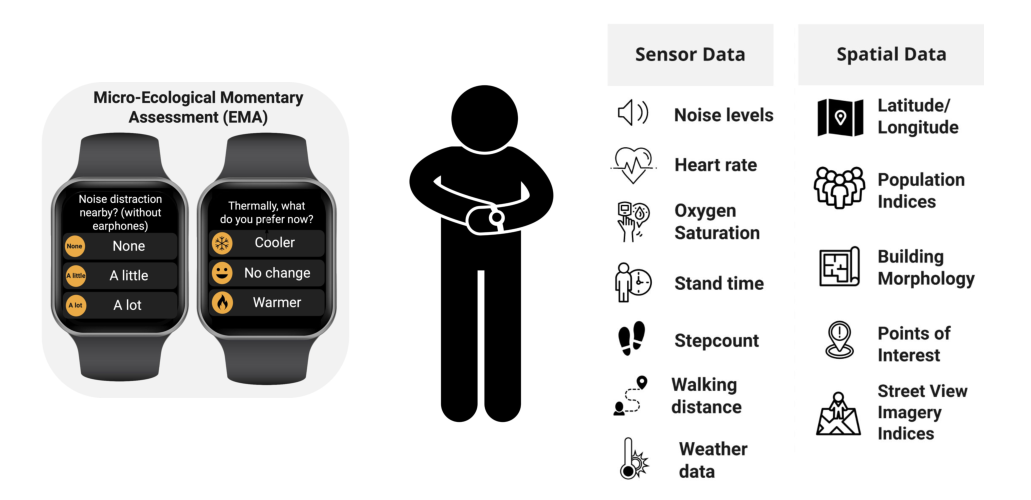
\includegraphics[width=0.92\textwidth]{figures/methods/cozie_study_design.pdf}
\caption{[PLACEHOLDER: Study design and data-collection workflow.]}
\label{fig:cozie-study-design}
\end{figure}

% [PLACEHOLDER: Describe the derived survey-level dataset
% (\texttt{cozie\_sg\_surveys\_with\_health\_aggregates}): 9{,}962 responses,
% 106 participants, 99+ columns. Explain how HealthKit physiological metrics are
% aggregated to a 1-hour pre-survey window and how home locations were recovered.]

% \subsubsection{Micro-survey structure}\label{sec:methods-perception}



% [PLACEHOLDER: List subjective variables --- thermal preference, noise level,
% noise kind, earphones, social context (alone/group), activity --- and their
% response categories.]

Each micro-survey is a short, branching battery answered directly on the watch face, shown in Figure~\ref{fig:cozie-microsurvey}.
A response records the participant's thermal preference (cooler, no change, or warmer) and the level of nearby noise (none, a little, or a lot); when noise is present, conditional follow-ups capture the kind of noise and whether earphones are being worn.
The survey also records the reported location or space type, the social context of being alone or in a group, and the activity being performed, with the available activity options depending on whether the participant is alone or with others.
Because several of these questions are conditional, later items such as noise kind and activity are answered only for the subset of responses that reach them, which produces the branching flow shown in Figure~\ref{fig:cozie-microsurvey}.

\begin{figure}[htbp]
\centering
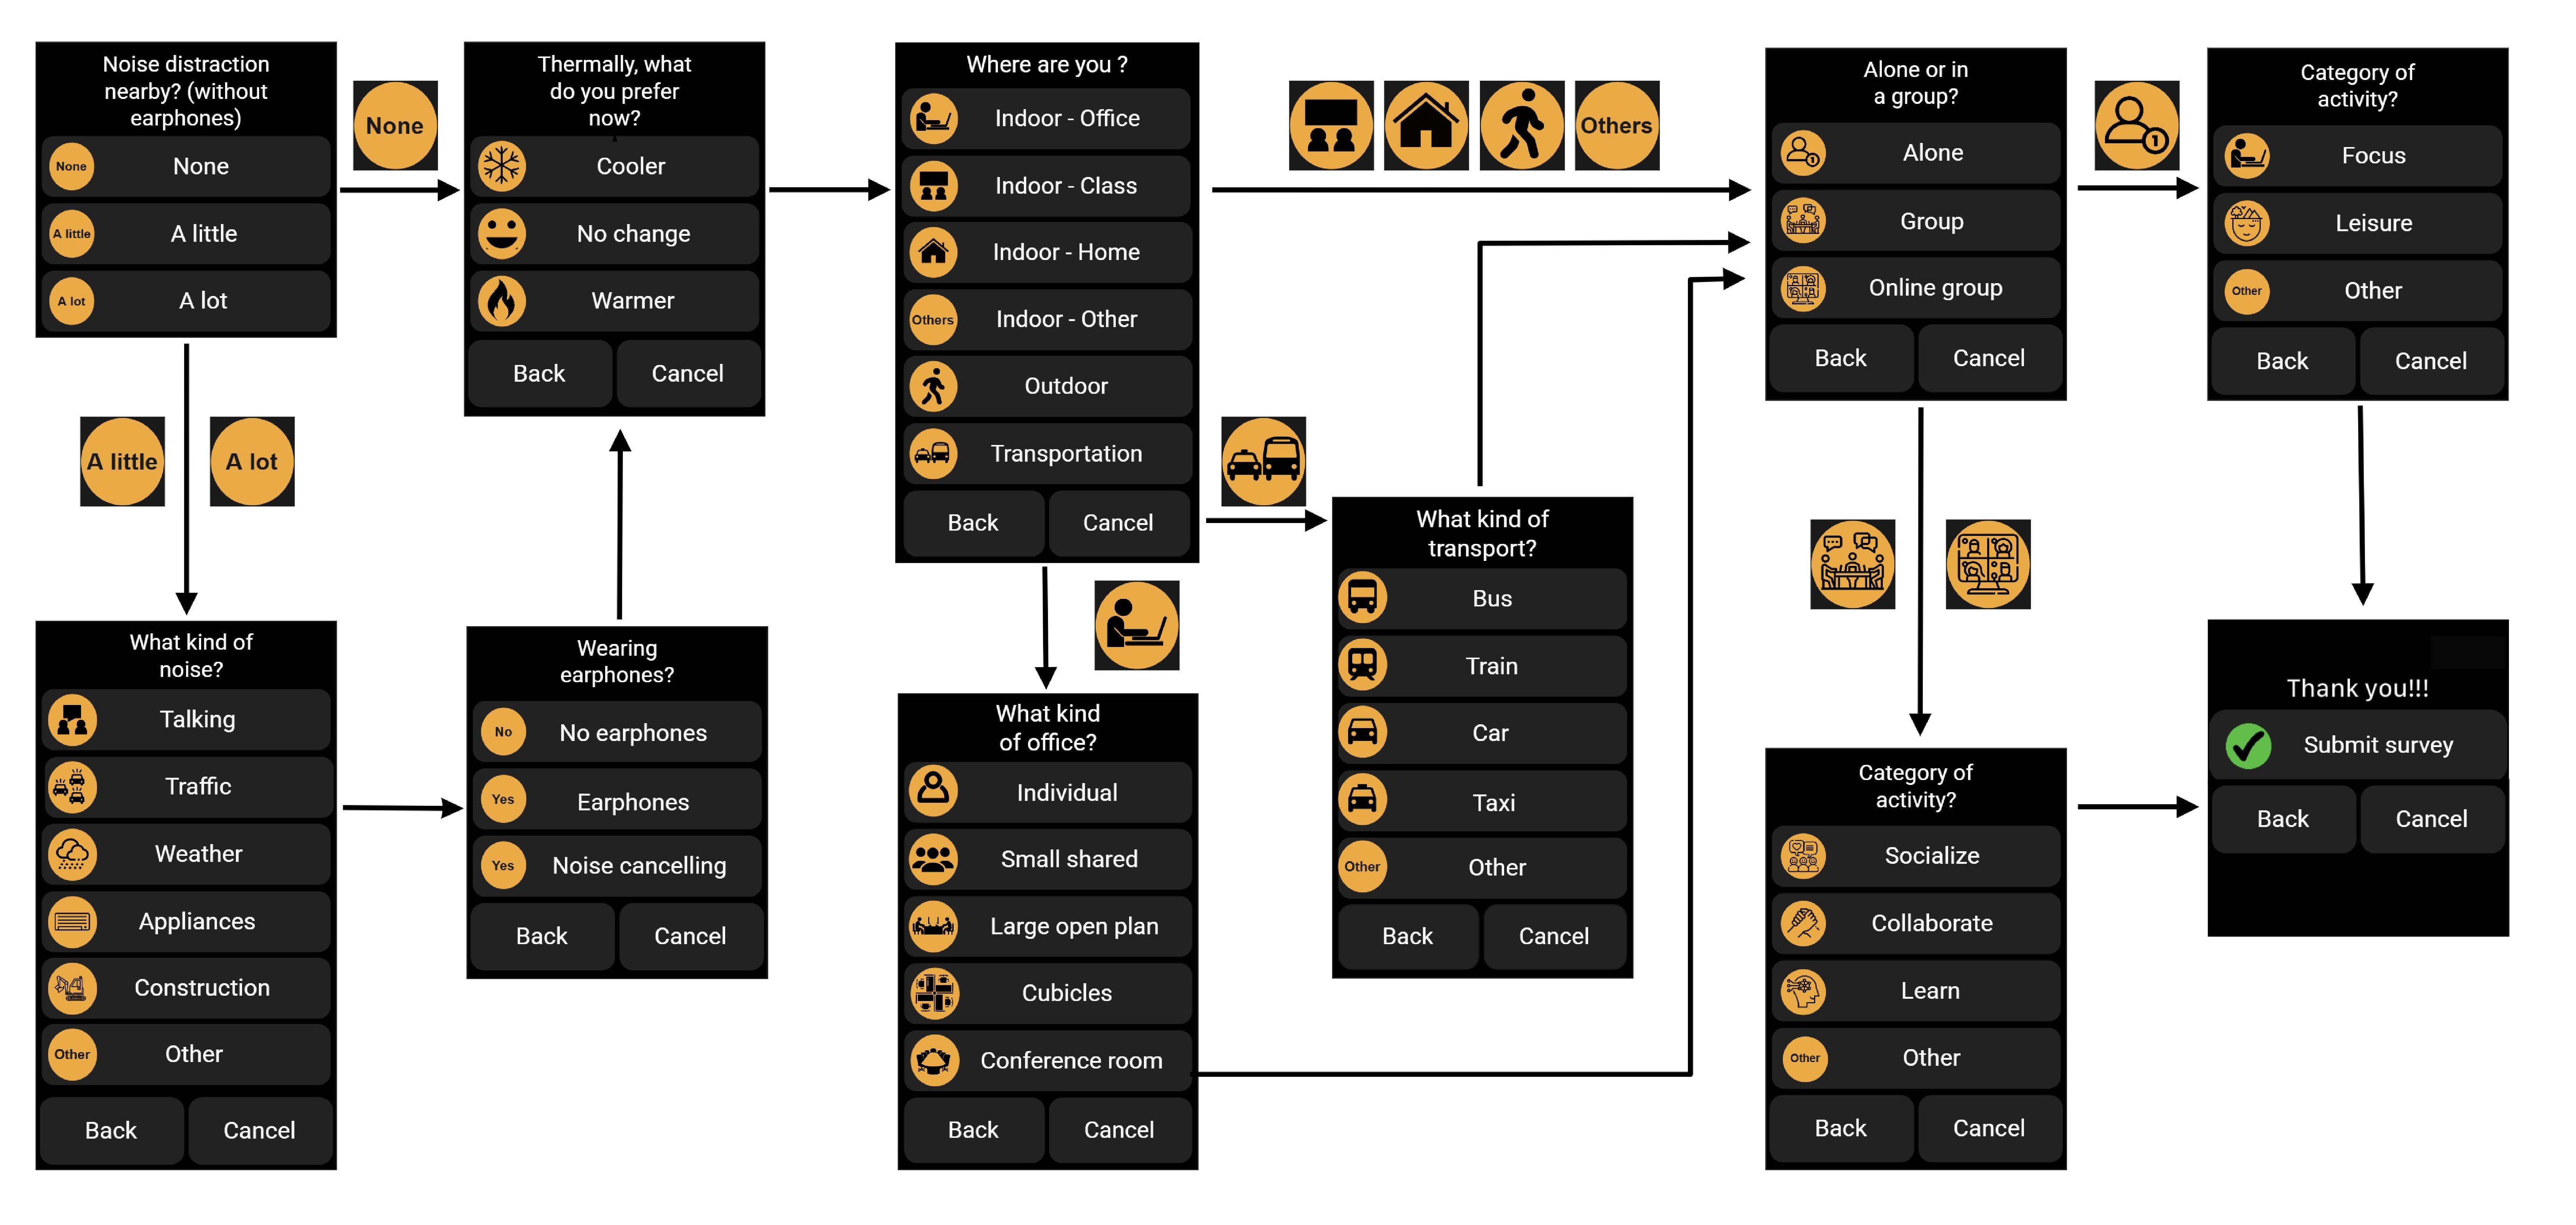
\includegraphics[width=0.92\textwidth]{figures/methods/cozie_microsurvey.pdf}
\caption{[PLACEHOLDER: Cozie smartwatch micro-survey interface and response flow.]}
\label{fig:cozie-microsurvey}
\end{figure}

% [PLACEHOLDER: Describe 1-hour aggregates --- mean heart rate, total steps,
% walking distance.]

Each geolocated response was also linked to a set of urban-context indicators derived with Urbanity, an open-source tool that builds feature-rich urban networks from open geospatial data \citep{Yap2023-xs}.
These indicators summarise the built environment around each response location, including streetscape view indices for greenery, sky, buildings, and roads, together with visual complexity, building count, population, and nearby points of interest across categories such as commercial, food, and recreational uses.
They provide the objective urban characterization used to test whether physical context adds information beyond the self-reported experience.

% \subsubsection{Weather data}\label{sec:methods-weather}
% [PLACEHOLDER: Describe the nearest-station weather aggregation --- air
% temperature, relative humidity, heat index, wind speed, rain, is-raining flag ---
% units and coverage (92--96\%). Note this is ambient, not skin-level, exposure.]

\subsection{Data processing and characterization}\label{sec:methods-eda}

% [PLACEHOLDER: Describe screening and merger of the data from the raw data set found in notebook 00]

The raw deployment data combine high-frequency watch and health streams with the sparser watch-survey responses in a single time-indexed record.
Survey responses were first screened to those triggered on the watch that carried valid, non-zero coordinates falling inside the Singapore bounding box, which produced the 9{,}962-response analysis set.
For each retained response, the seven temporal watch-health streams were aggregated over three pre-survey windows of six hours, one hour, and ten minutes, summarising each window by its count, mean, spread, and extremes, and by an accumulated total for step count, walking distance, and stand time.
The nearest weather-station observations were aggregated over the same three windows, and a heat index was derived from air temperature and relative humidity.
These health and weather aggregates were then merged back onto the survey rows and checked for consistency, yielding one analysis-ready record per response that carries the original survey and location fields alongside the linked physiological, weather, and urban-context features used throughout the analysis.

[PLACEHOLDER: Describe the EDA strategy from notebook 01 --- univariate survey /
health distributions, thermal relationships, temporal profiling in Singapore
local time, and geospatial mapping.]

[PLACEHOLDER: Describe the characterization methods from notebook 01 ---
perception fingerprints (row-normalized conditional proportions and lift),
association and effect size (Kruskal--Wallis $\varepsilon^2$, chi-square /
Cram\'er's V, Spearman $\rho$)



% ============================================================================
\section{Results}\label{sec:results}
% ============================================================================

\subsection{Data collection, coverage, and temporal characteristics}\label{sec:res-data-collection}
[PLACEHOLDER: Describe how the study data were collected across Singapore, including geographic coverage, response volume, participant engagement, and the temporal distribution of responses. Explain the weekly and space-type-specific timing patterns that establish the context for the analyses that follow.]

\begin{figure}[htbp]
\centering
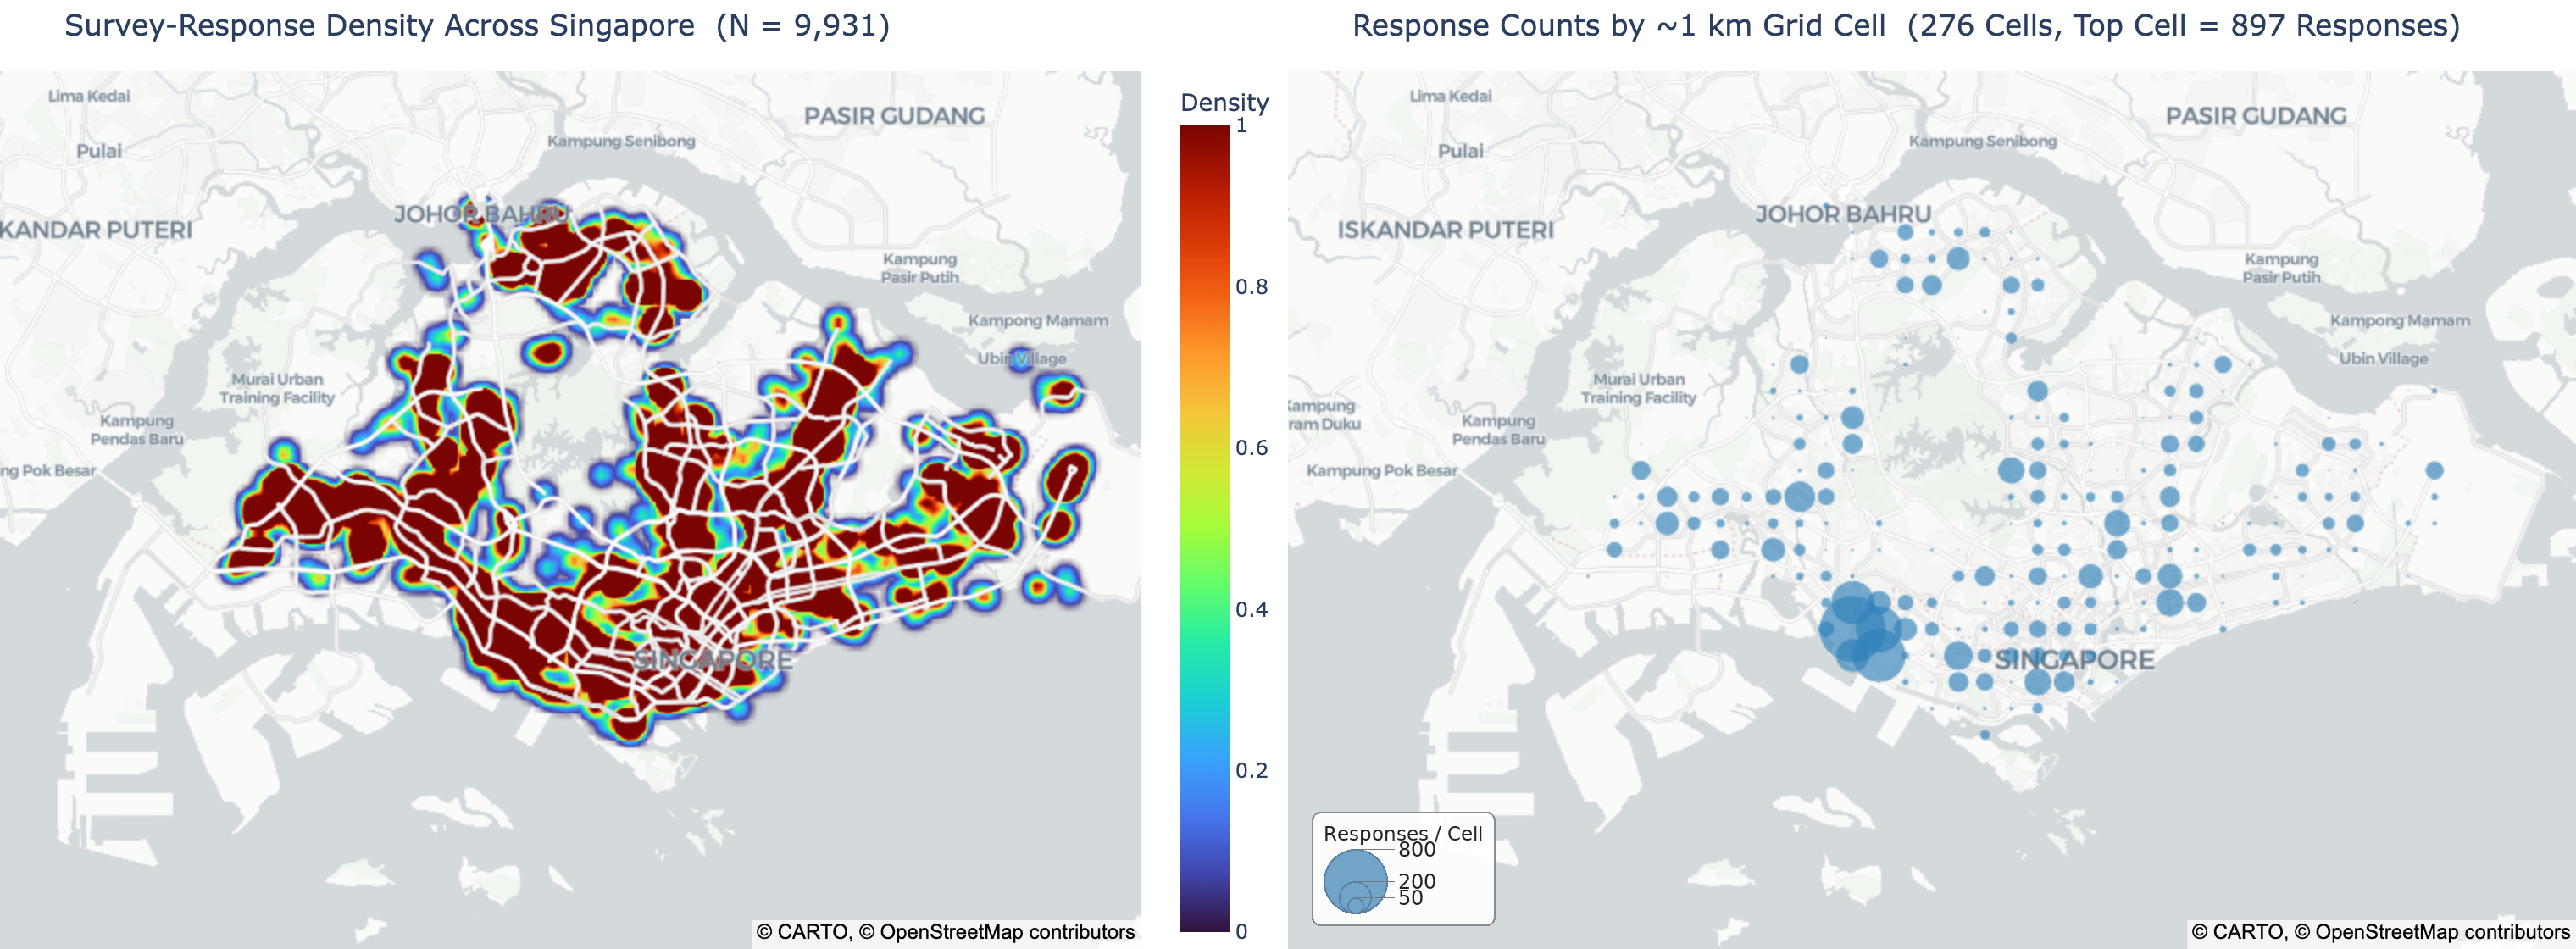
\includegraphics[width=\textwidth]{figures/data_characterization/response_density_and_grid_counts.png}
\caption{[PLACEHOLDER: Survey-response density and response counts by approximately 1-km grid cell across Singapore (Figure B4).]}
\label{fig:data-b4-response-density-grid-counts}
\end{figure}

\begin{figure}[htbp]
\centering
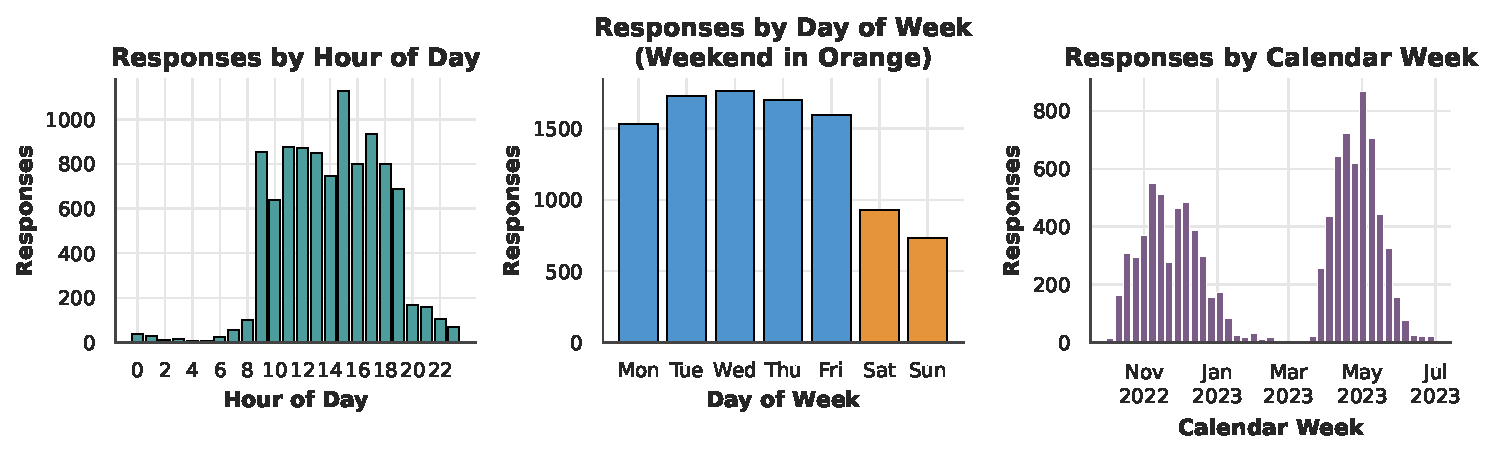
\includegraphics[width=\textwidth]{figures/data_characterization/weekly_temporal_cadence.pdf}
\caption{[PLACEHOLDER: Weekly temporal cadence of survey responses in Singapore local time (Figure D2).]}
\label{fig:data-d2-temporal-cadence}
\end{figure}

\begin{figure}[htbp]
\centering
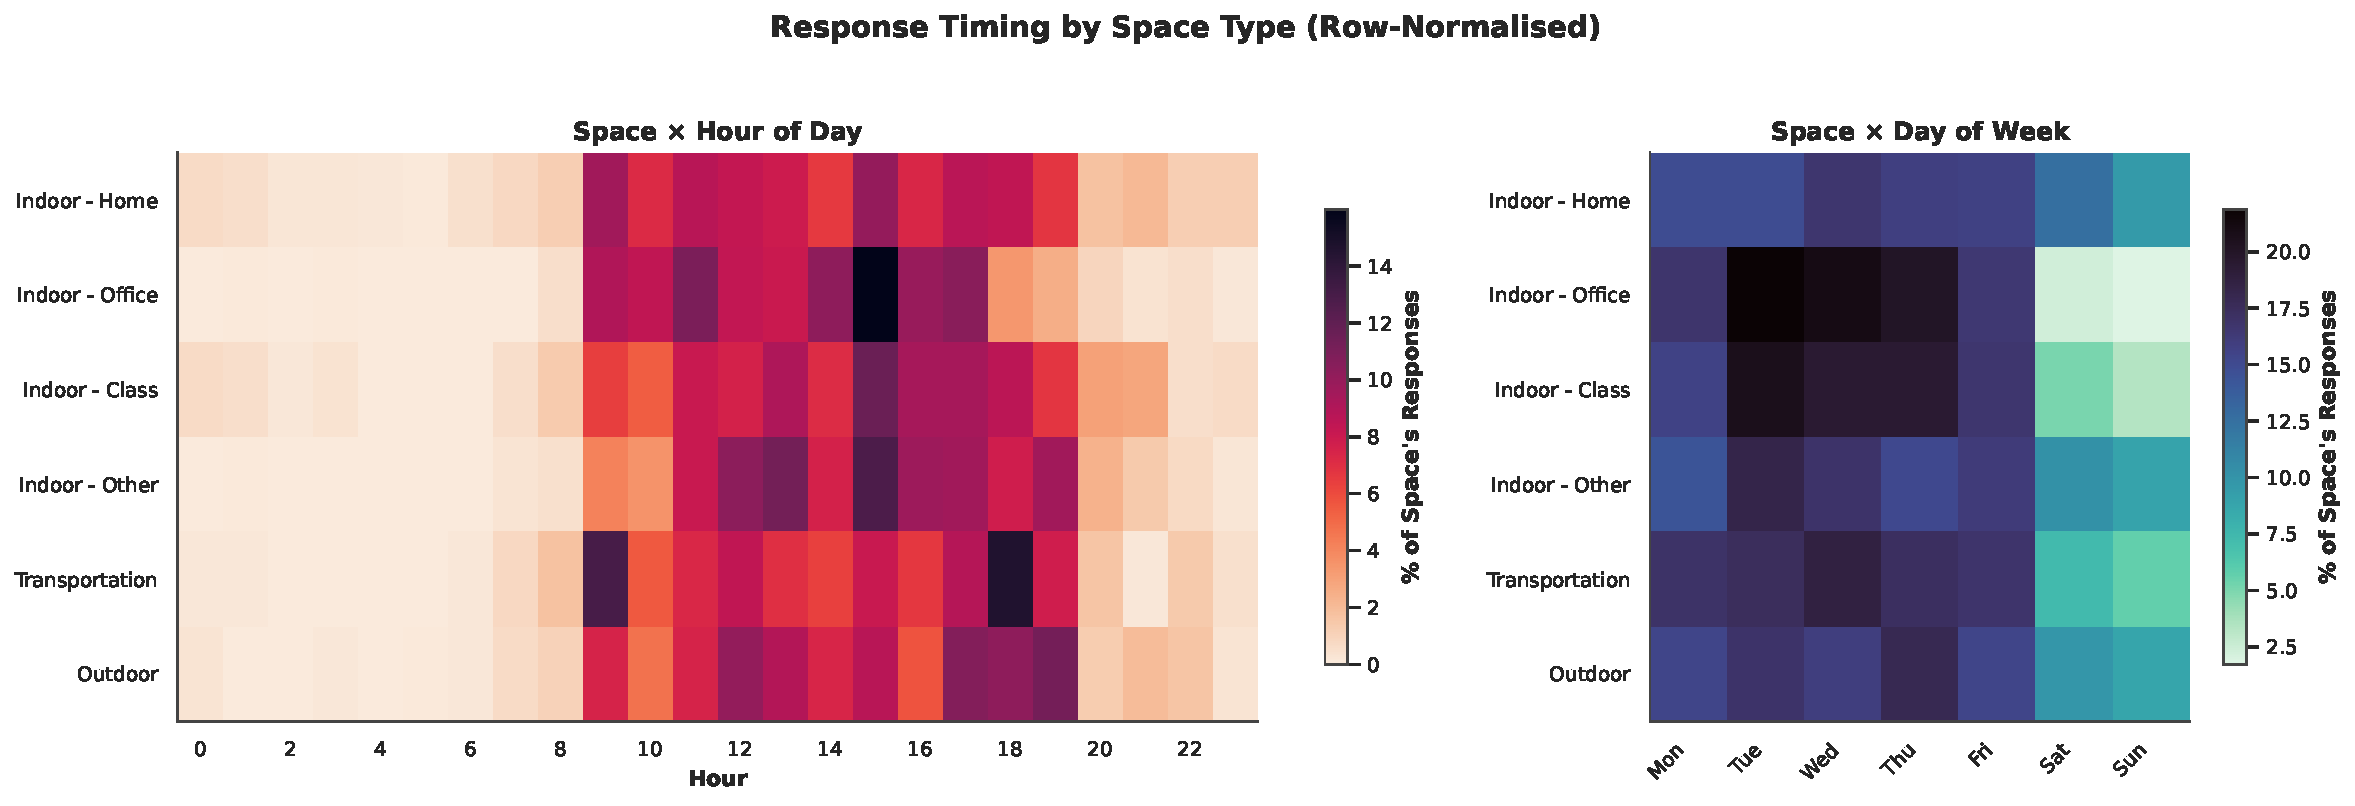
\includegraphics[width=\textwidth]{figures/data_characterization/space_type_timing_heatmaps.pdf}
\caption{[PLACEHOLDER: Response timing by space type, shown by hour of day and day of week (Figure D4).]}
\label{fig:data-d4-space-time}
\end{figure}

\begin{figure}[htbp]
\centering
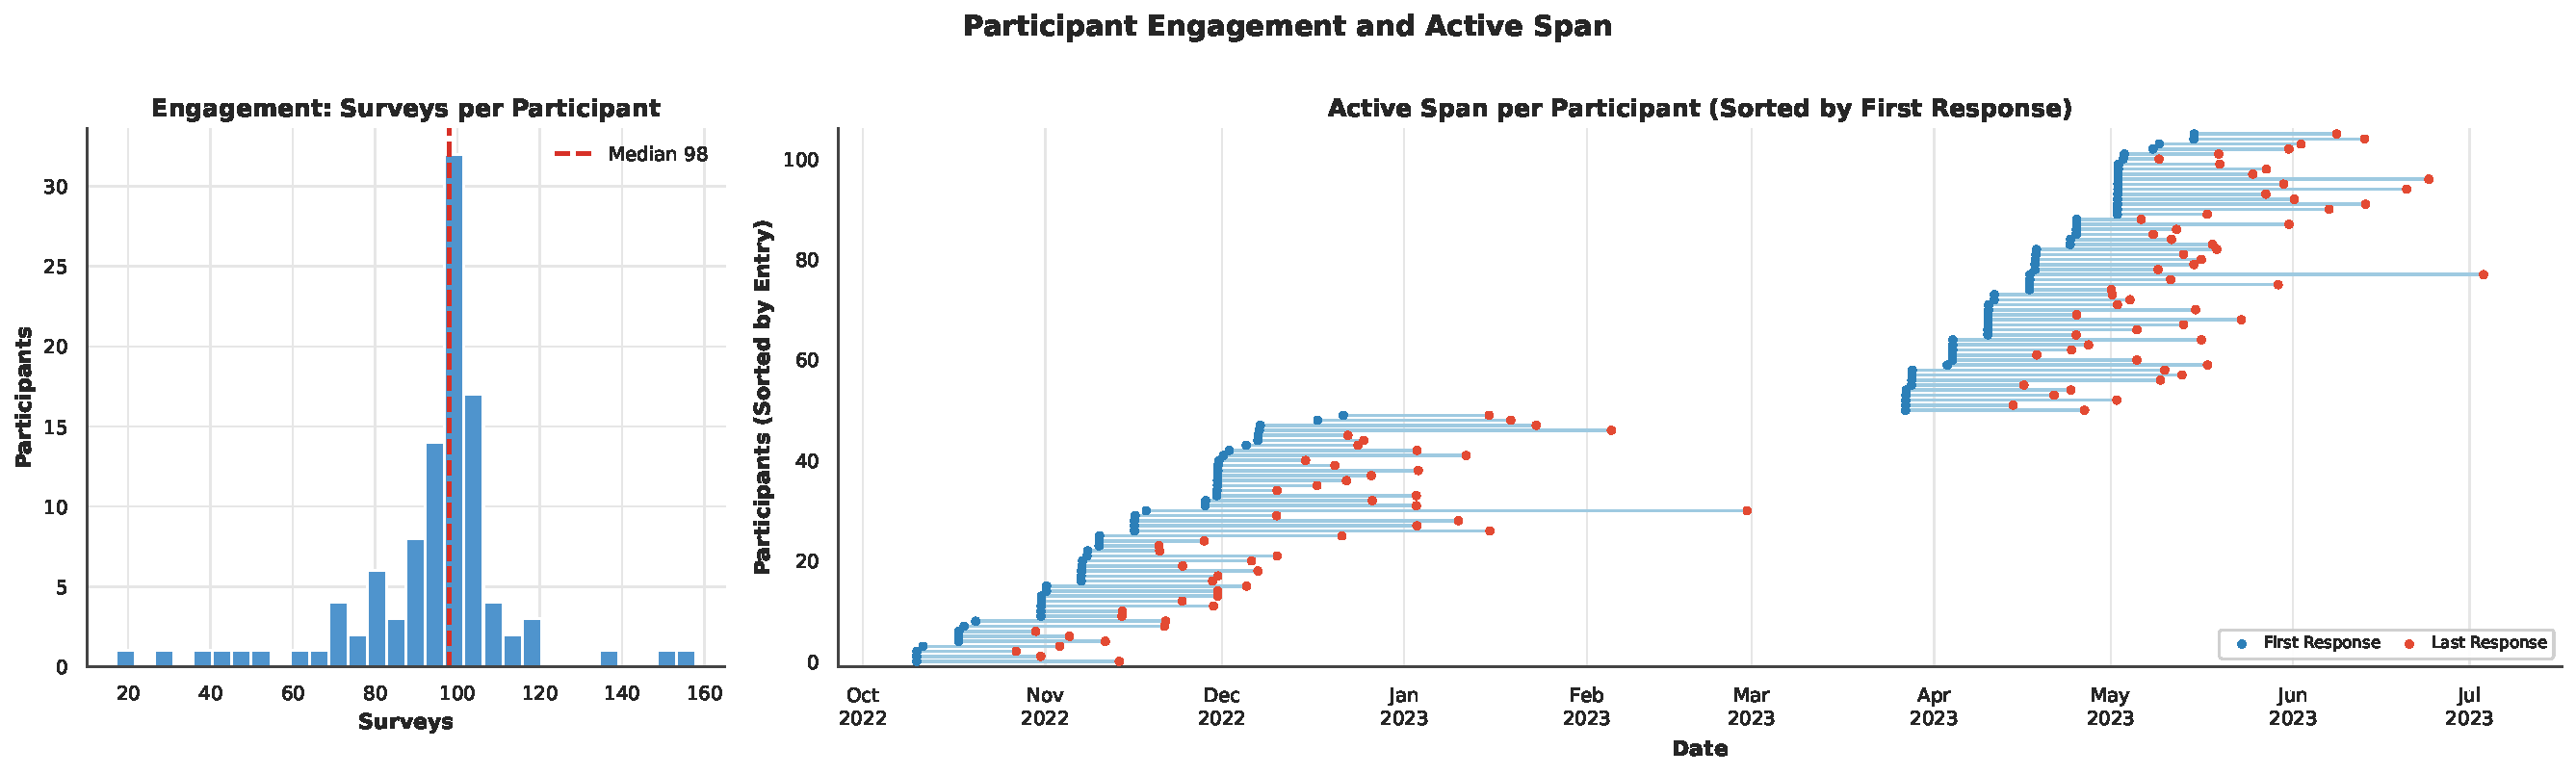
\includegraphics[width=\textwidth]{figures/data_characterization/participant_engagement.pdf}
\caption{[PLACEHOLDER: Participant engagement and active survey span (Figure E2).]}
\label{fig:data-e2-engagement}
\end{figure}

\subsection{Survey responses and linked temporal data coverage}\label{sec:res-survey-overview}
[PLACEHOLDER: Summarize the survey battery, response coverage, and the main conditional paths through the questionnaire. Describe the coverage and distributions of linked wearable-health and nearest-station weather observations across the pre-survey aggregation windows.]

\begin{figure}[htbp]
\centering
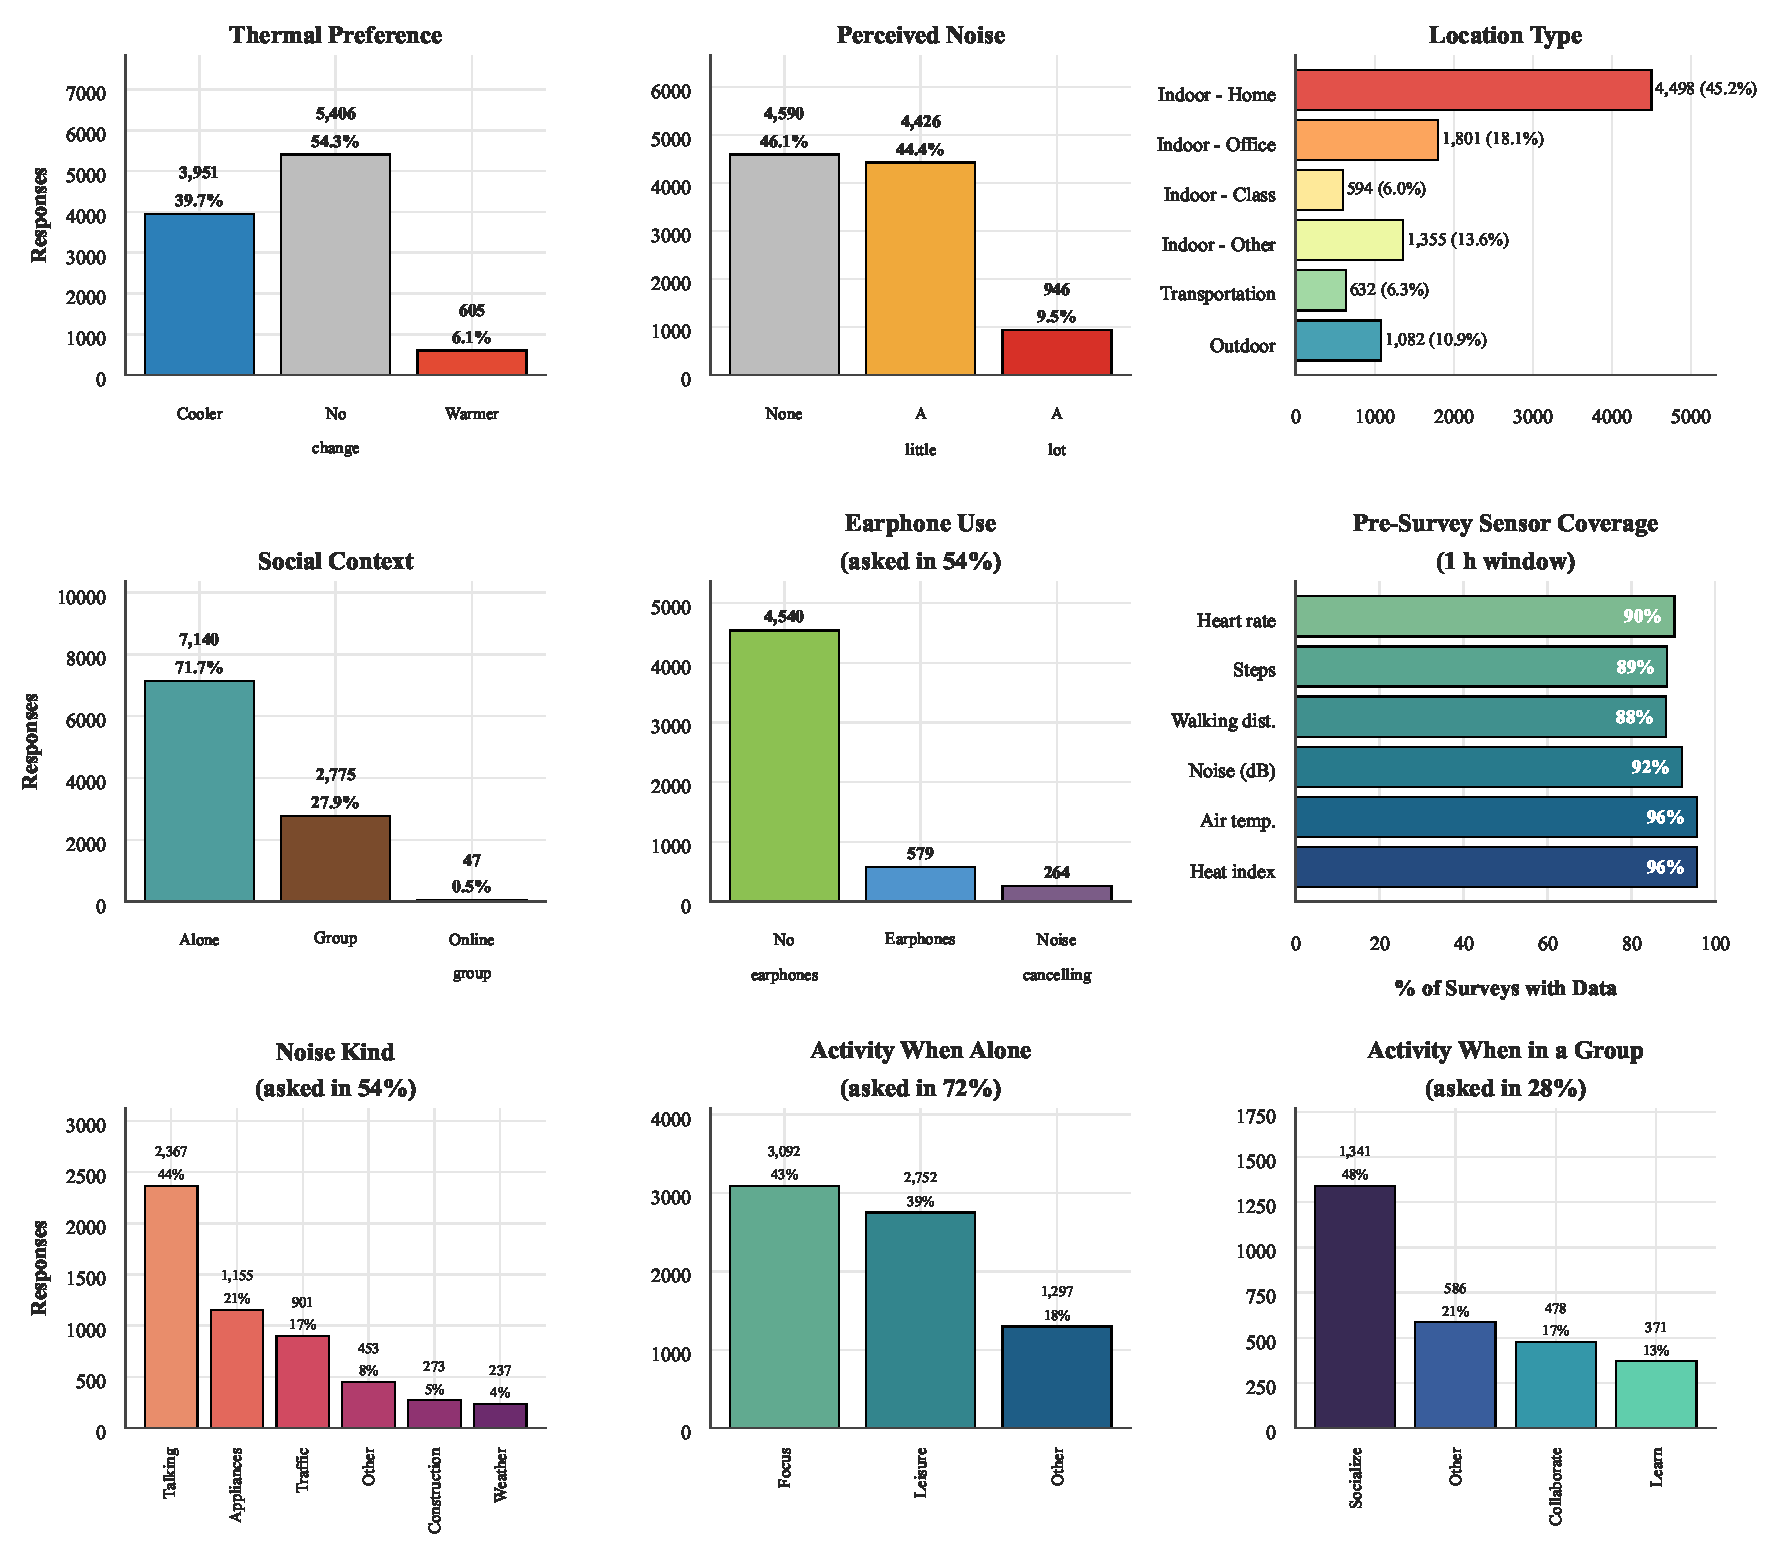
\includegraphics[width=\textwidth]{figures/data_characterization/survey_battery_and_coverage.pdf}
\caption{[PLACEHOLDER: Survey response battery, conditional follow-ups, and linked-sensor coverage (Figure A1).]}
\label{fig:data-a1-survey-battery}
\end{figure}

\begin{figure}[htbp]
\centering
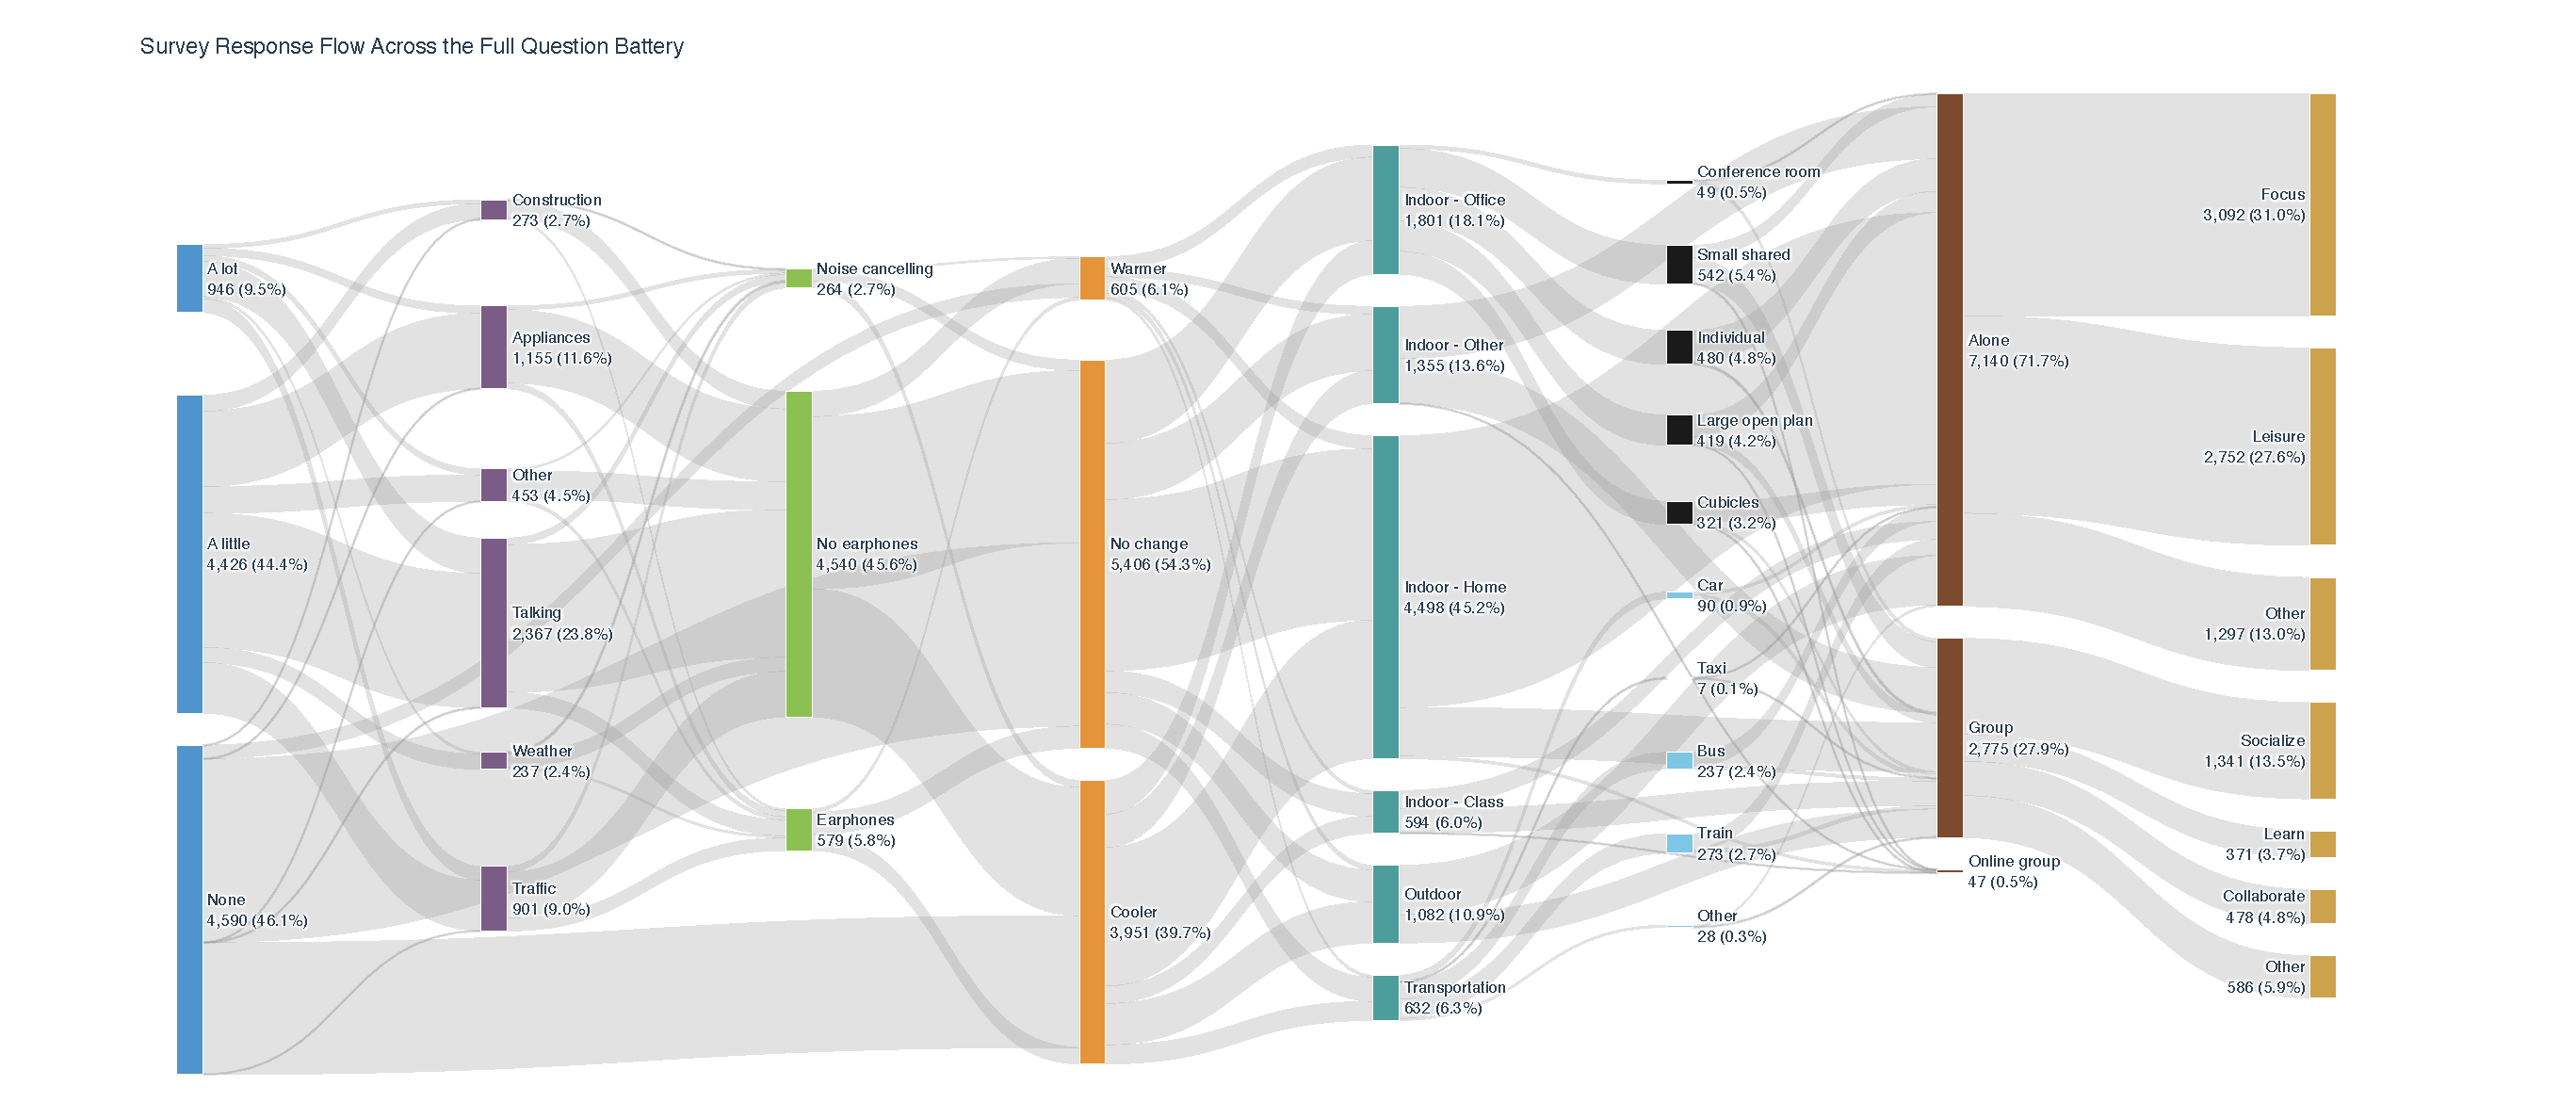
\includegraphics[width=\textwidth]{figures/data_characterization/survey_response_flow.pdf}
\caption{[PLACEHOLDER: Conditional response flow through the watch-survey questionnaire.]}
\label{fig:survey-response-flow}
\end{figure}

\begin{figure}[htbp]
\centering
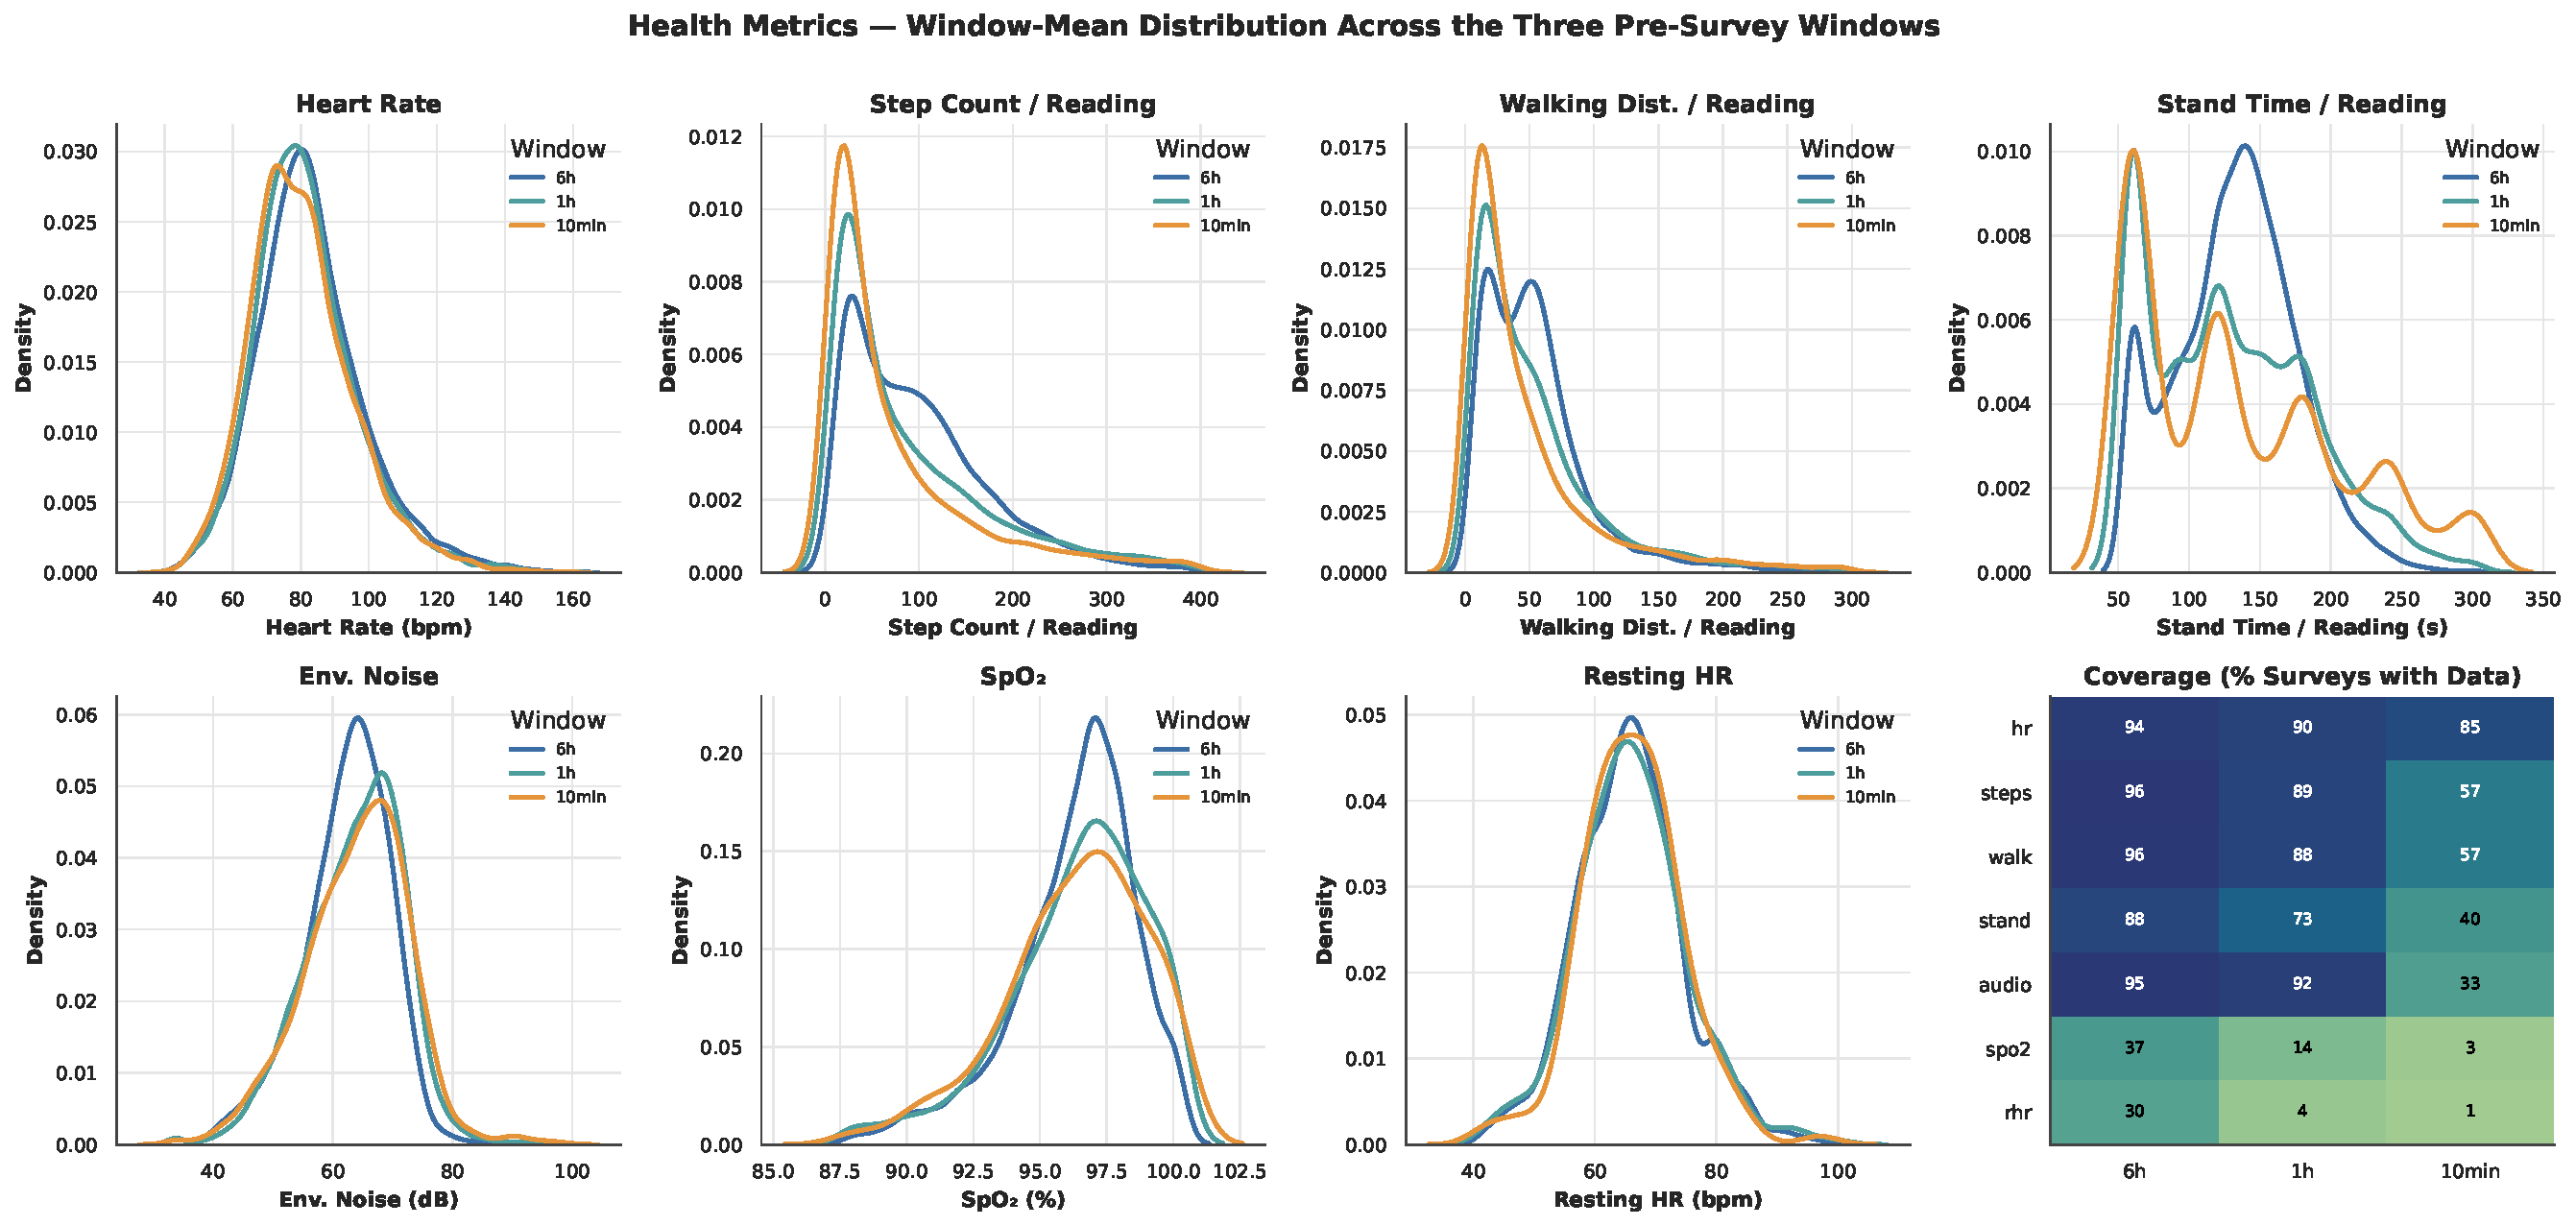
\includegraphics[width=\textwidth]{figures/data_characterization/wearable_health_windows.pdf}
\caption{[PLACEHOLDER: Wearable-health metrics across pre-survey aggregation windows (Figure A2).]}
\label{fig:data-a2-health-windows}
\end{figure}

\begin{figure}[htbp]
\centering
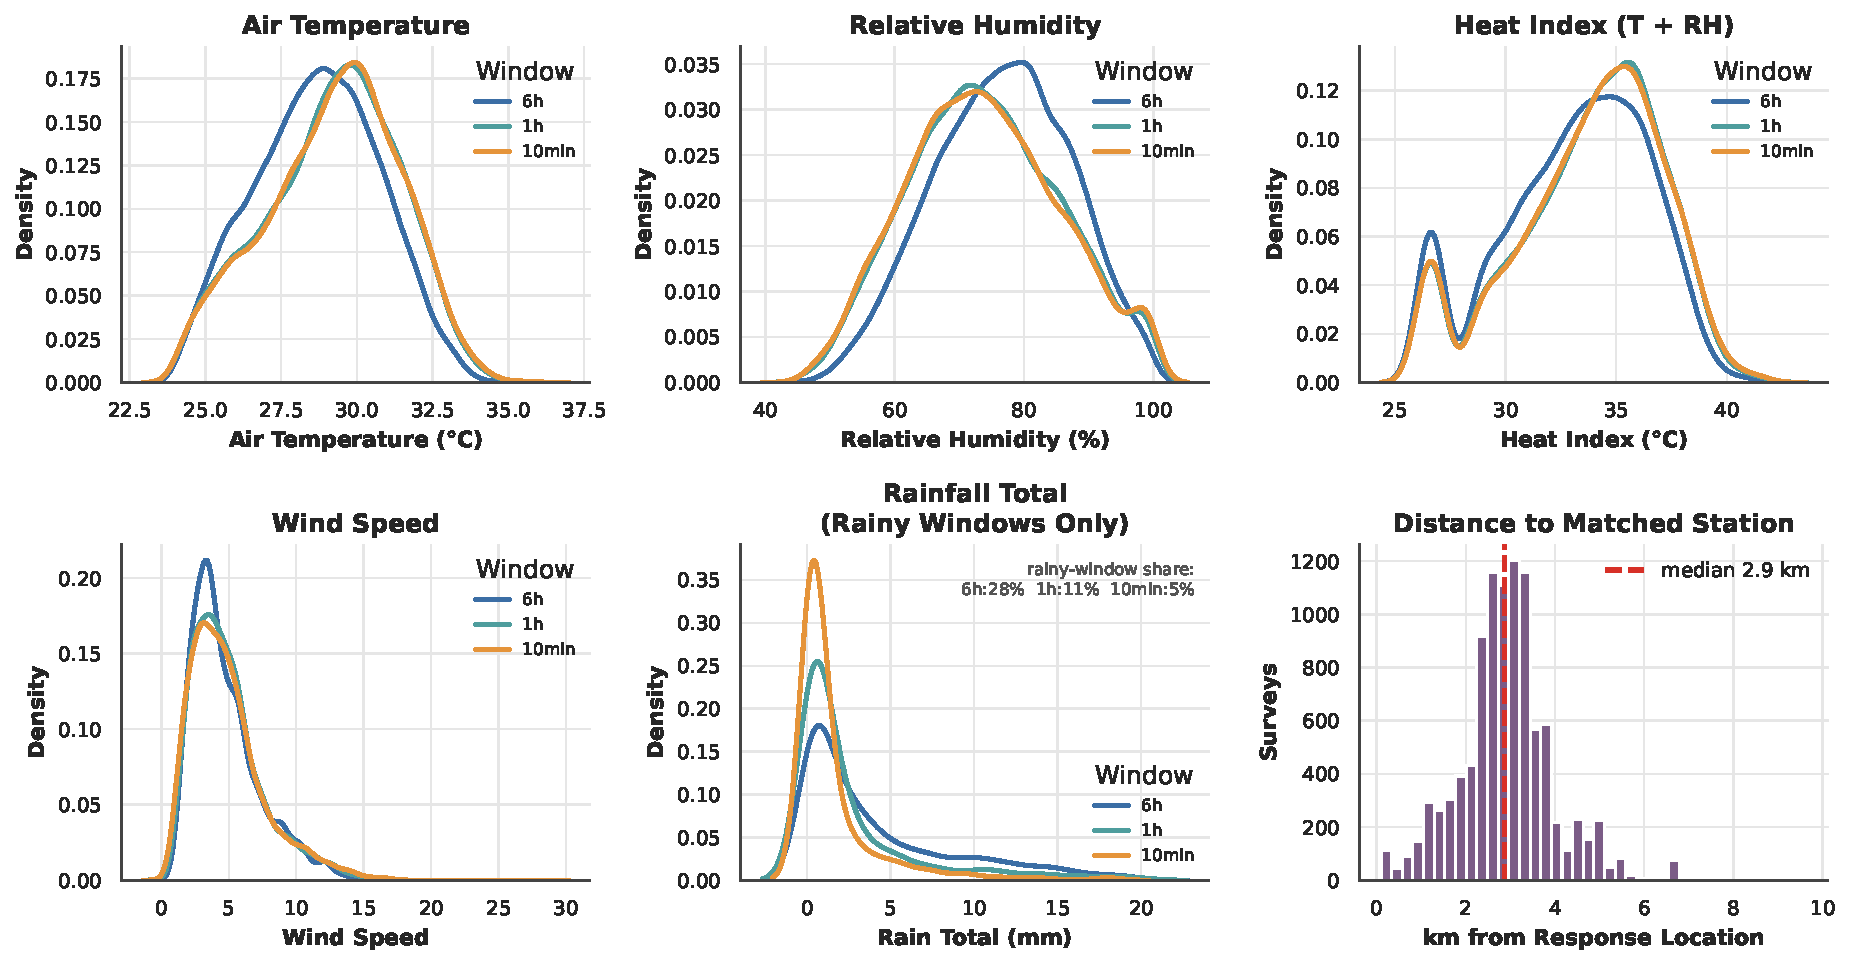
\includegraphics[width=\textwidth]{figures/data_characterization/outdoor_weather_windows.pdf}
\caption{[PLACEHOLDER: Nearest-station outdoor ambient weather across pre-survey aggregation windows (Figure A3).]}
\label{fig:data-a3-weather-windows}
\end{figure}

\subsection{Thermal preference and noise characterization}\label{sec:res-thermal-noise}
[PLACEHOLDER: Provide an overview of thermal preference and acoustic experience across participants, contexts, and reported locations. Explain what the cooling-preference and noise-characterization figures establish about the distribution of these outcomes before examining their relationships with space type.]

\begin{figure}[htbp]
\centering
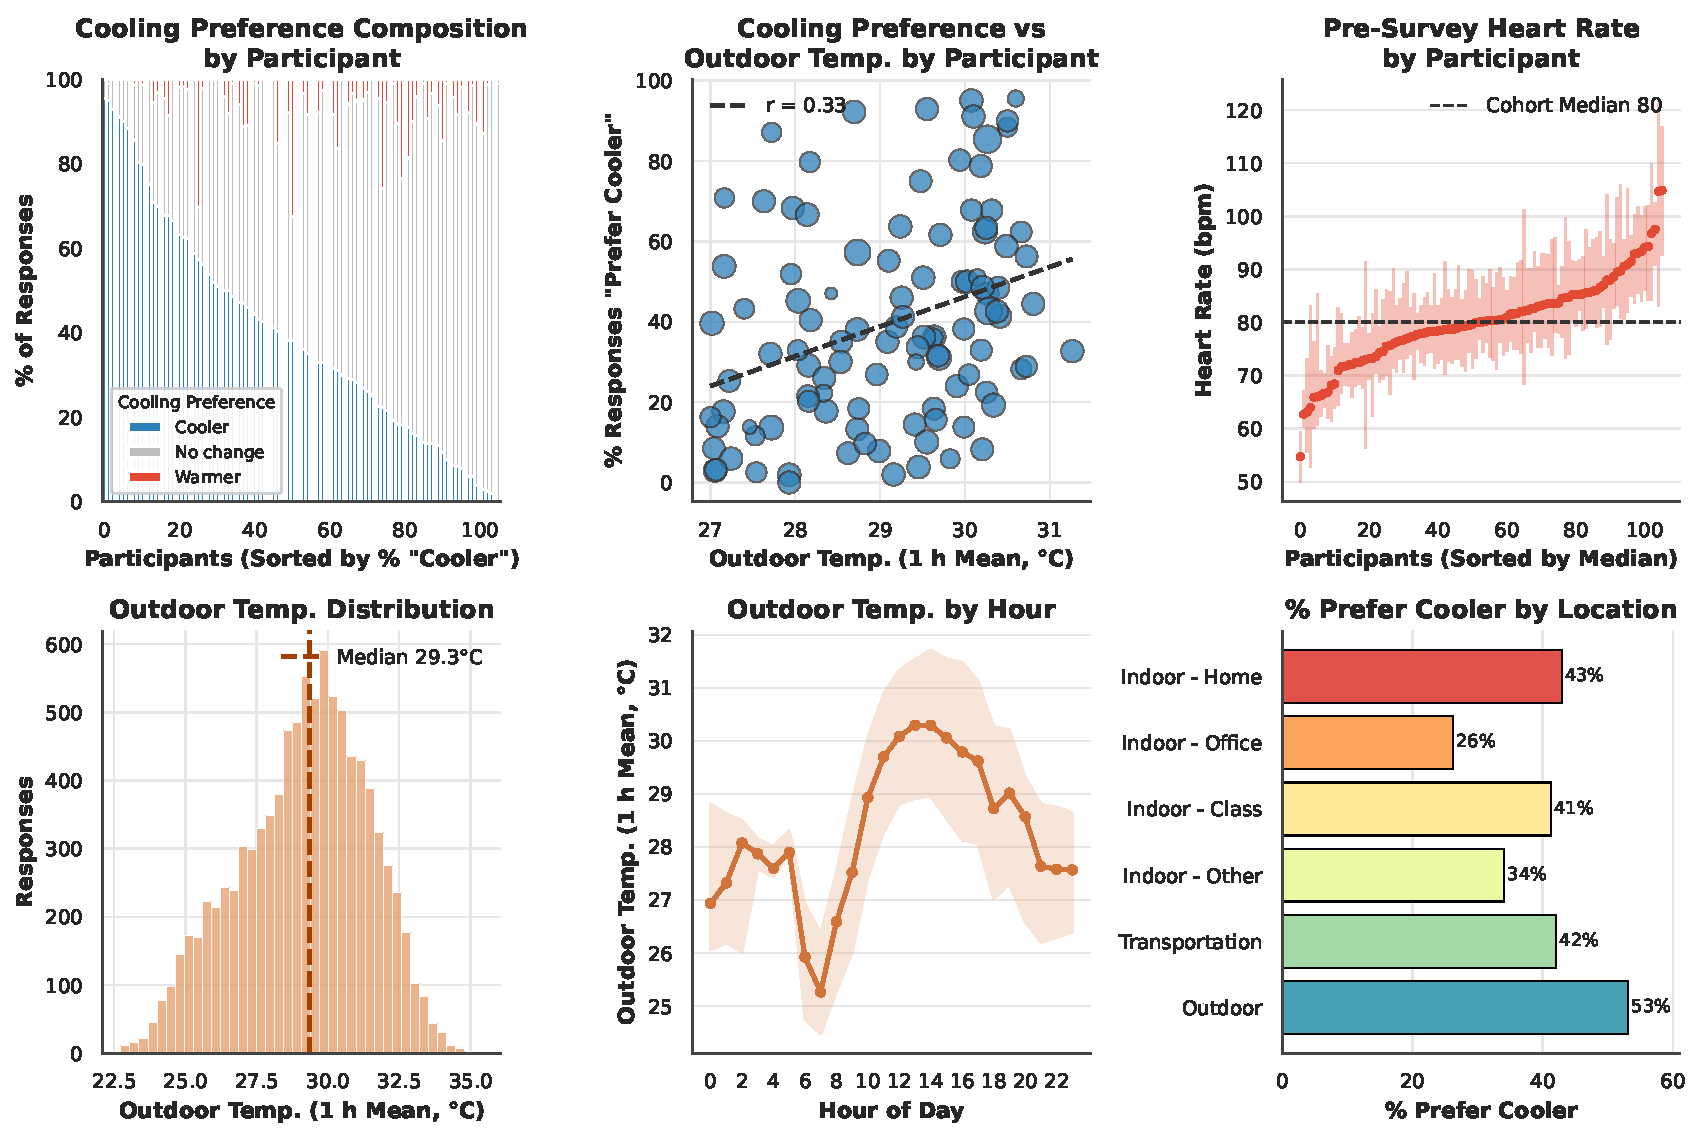
\includegraphics[width=\textwidth]{figures/data_characterization/cooling_preference.pdf}
\caption{[PLACEHOLDER: Participant-level and contextual patterns in cooling preference (Figure F2).]}
\label{fig:data-f2-cooling}
\end{figure}

% The source notebook identifies this visualization as Figure G1 (not G2).
\begin{figure}[htbp]
\centering
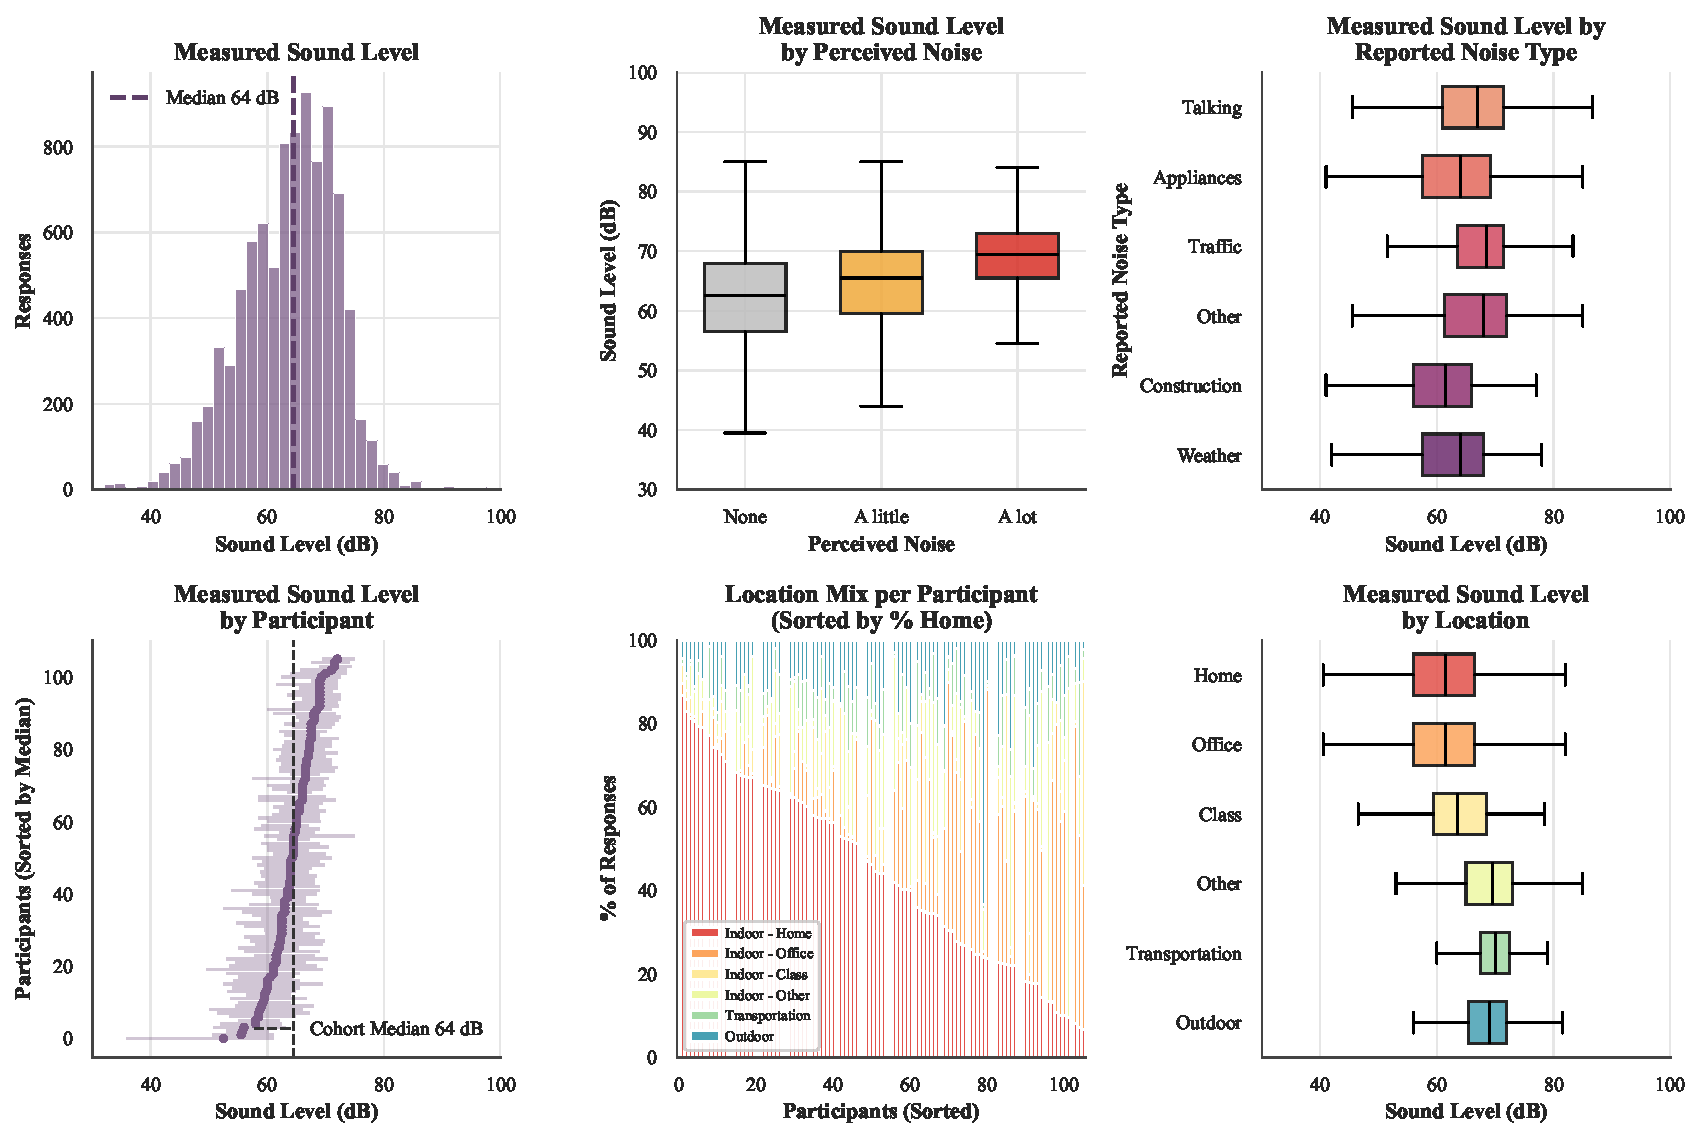
\includegraphics[width=\textwidth]{figures/data_characterization/noise_characterization.pdf}
\caption{[PLACEHOLDER: Measured sound level across subjective, participant, and location contexts (Figure G1).]}
\label{fig:data-g1-noise}
\end{figure}

\subsection{Perceptual fingerprints and association with space type}\label{sec:res-fingerprint-association}

[PLACEHOLDER: Explain the conditional perception profiles in Figure~\ref{fig:space-perception-fingerprint}. Identify the dominant response patterns within each space type across thermal preference, noise, earphone use, social context, and activity. Make clear that each row is normalized within a space type, so values describe the composition of experiences reported in that space rather than absolute response volume.]

\begin{figure}[htbp]
\centering
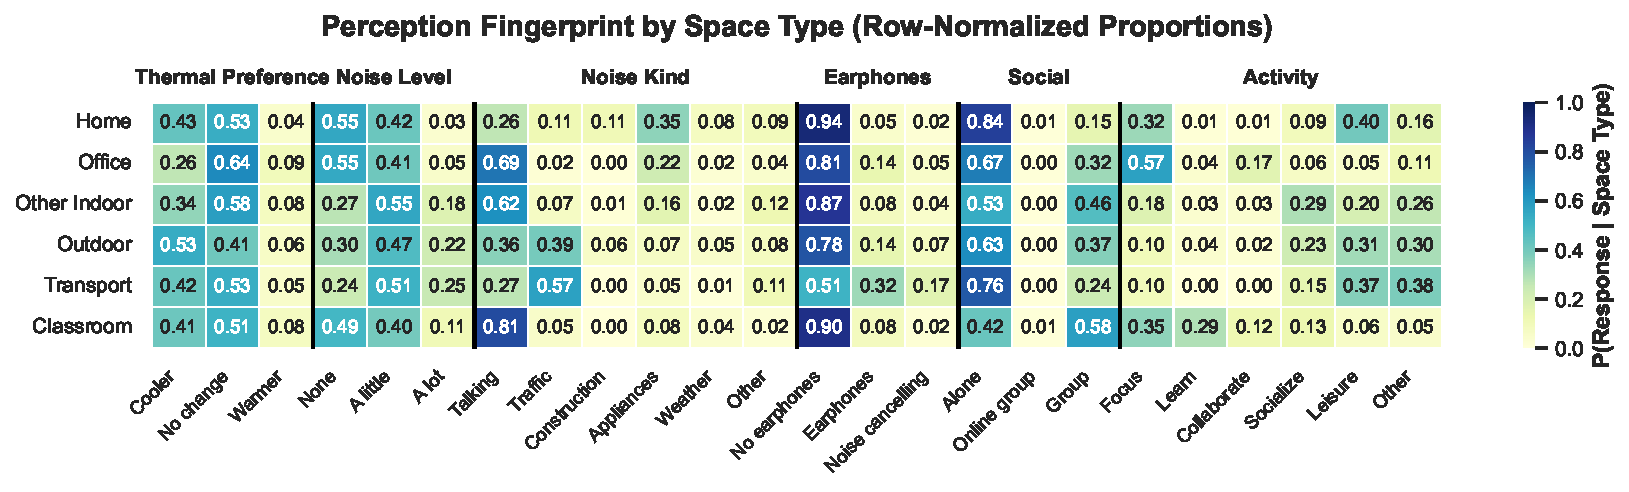
\includegraphics[width=\textwidth]{figures/data_characterization/perception_fingerprint_by_space_type.pdf}
\caption{[PLACEHOLDER: Conditional perception fingerprint by reported space type (Figure A1). Cells show $P(\mathrm{response}\mid\mathrm{space\ type})$.]}
\label{fig:space-perception-fingerprint}
\end{figure}

[PLACEHOLDER: Explain the relative distinctiveness in Figure~\ref{fig:space-perception-lift}. Highlight response patterns that are over-represented or under-represented relative to the full survey corpus, and distinguish these relative contrasts from the raw within-space proportions in Figure~\ref{fig:space-perception-fingerprint}.]

\begin{figure}[htbp]
\centering
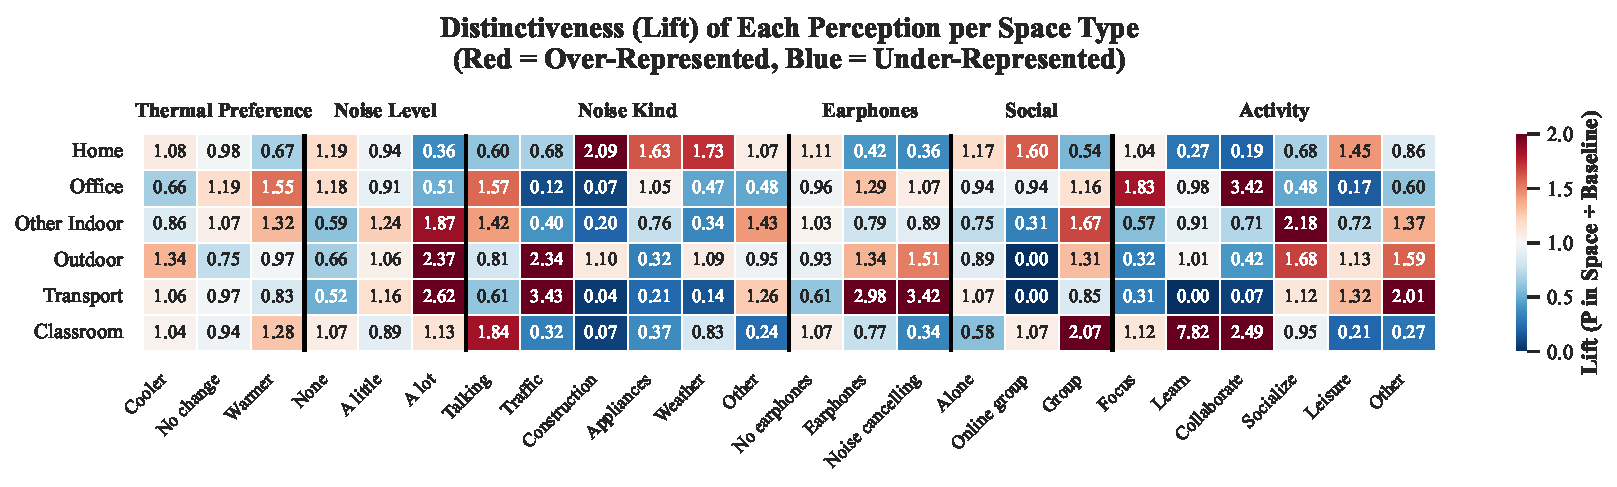
\includegraphics[width=\textwidth]{figures/data_characterization/perception_lift_by_space_type.pdf}
\caption{[PLACEHOLDER: Relative distinctiveness of perceptions by reported space type (Figure A2). Cells show lift, $P(\mathrm{response}\mid\mathrm{space\ type}) / P(\mathrm{response})$.]}
\label{fig:space-perception-lift}
\end{figure}

[PLACEHOLDER: Interpret the cell-level contrasts in Figure~\ref{fig:space-perception-residuals}. Identify the space--response combinations that occur more or less often than expected under independence, focus on coherent patterns across related variables, and treat the significance markers as descriptive screens because responses are nested within participants.]

\begin{figure}[htbp]
\centering
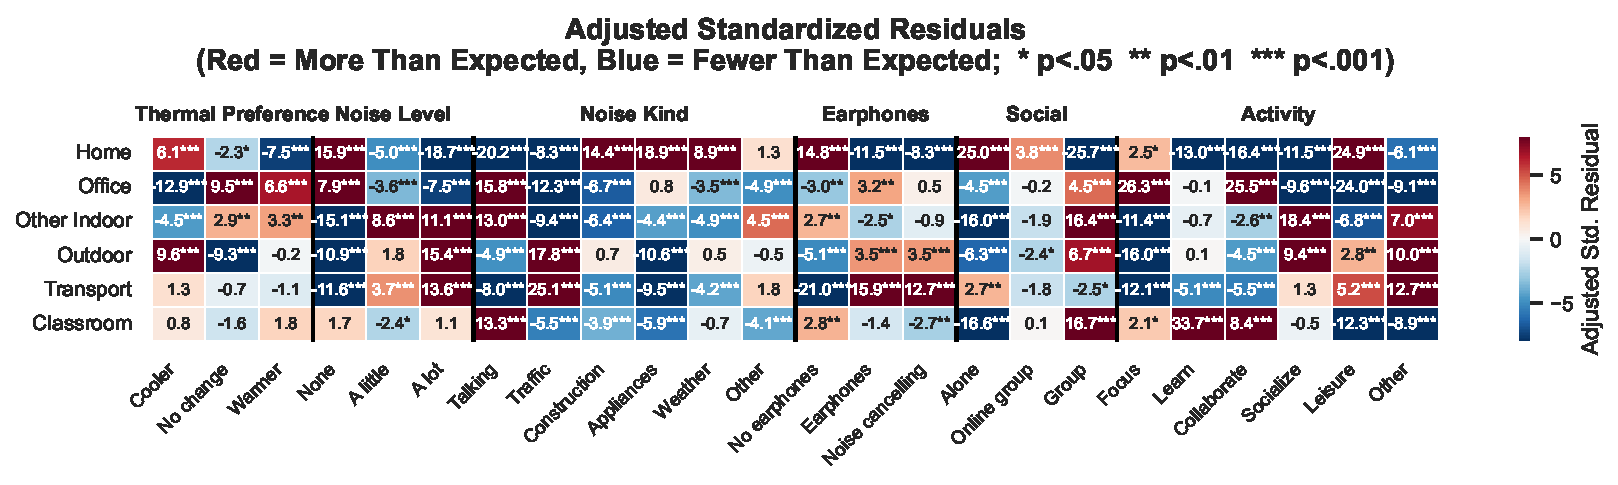
\includegraphics[width=\textwidth]{figures/data_characterization/perception_space_adjusted_residuals.pdf}
\caption{[PLACEHOLDER: Adjusted standardised residuals for space type and perceptual-response combinations (Figure B2). Red cells occur more often than expected under independence and blue cells occur less often than expected.]}
\label{fig:space-perception-residuals}
\end{figure}

\subsection{Multivariate, physiological, weather, and outdoor environmental patterns}\label{sec:res-multivariate-physio-outdoor}
[PLACEHOLDER: Integrate the multivariate structure of subjective experience (MCA + k-modes) with physiological and weather signatures across space types. Then describe the outdoor-only environmental characterization, including streetscape and built-form profiles, their relationship with thermal preference, and the role of weather.]

[PLACEHOLDER: Report the physiological gradient across spaces (sedentary Home to mobile Outdoor/Transport; steps largest effect), the weak ambient-weather signatures of space type, and the result that Outdoor is not necessarily the hottest reported space.]

[PLACEHOLDER: Report the weather-versus-thermal-preference result: ``Cooler'' responses occur in genuinely hotter (higher heat-index) and drier conditions, while rain suppresses cooling demand. State the magnitude and limitations of this relationship.]


% \subsection{Discriminative modeling of space type}\label{sec:res-model}
% [PLACEHOLDER: Report the space-type classifier performance and feature importance
% (activity and noise-kind as strong space descriptors; ambient weather adds little).]


% ============================================================================
\section{Discussion}\label{sec:discussion}
% ============================================================================

\subsection{Principal findings}\label{sec:disc-findings}
[PLACEHOLDER: Synthesize: function/behaviour (activity, noise + coping, movement)
separates space types robustly; thermal, environmental and physiological
expectations are mostly weak or convergent nulls; the weather correction shows
ambient weather is nearly useless for identifying a space yet genuinely drives
outdoor thermal preference.]

\subsection{Interpretation against intuition}\label{sec:disc-intuition}
[PLACEHOLDER: Discuss the reinforced vs contradicted intuitions (e.g. Outdoor is
not the hottest; streetscape greenery does not move thermal preference; actual
heat does).]

\subsection{Implications for sustainable urban design}\label{sec:disc-implications}
[PLACEHOLDER: Connect findings to the journal scope --- what they mean for
thermal-comfort-aware, health-supportive and energy-conscious urban design and
policy in tropical cities.]

\subsection{Limitations}\label{sec:disc-limitations}
[PLACEHOLDER: Participant nesting / pseudoreplication; ambient nearest-station
weather as a coarse proxy for personal exposure; convenience sample; Singapore-
specific A/C context; self-reported perceptions.]

\subsection{Future work}\label{sec:disc-future}
[PLACEHOLDER: Directions --- personal microclimate sensing, larger/more diverse
cohorts, cross-city replication, mixed-effects modeling accounting for
participant nesting.]


% ============================================================================
\section{Conclusion}\label{sec:conclusion}
% ============================================================================
[PLACEHOLDER: Concise restatement of the contribution and headline takeaway for
sustainable urban development.]


% ============================================================================
\section*{Acknowledgements}
% ============================================================================
The authors acknowledge the student researchers who assisted with data collection and processing: Charis Boey, Kristi Maisha, Annabel Sim, Aisyah Iskandar, Lum Jun Chao, and S Aravindkugesh.

\section*{CRediT authorship contribution statement}
Clayton Miller: Visualization, Software, Resources, Methodology, Funding acquisition, Formal analysis, Writing -- original draft, Supervision, Project administration, Investigation, Conceptualization. Yun Xuan Chua: Methodology, Conceptualization, Writing -- review \& editing, Project administration, Investigation. Mario Frei: Writing -- review \& editing, Validation, Project administration, Investigation, Conceptualization, Methodology, Data curation.

\section*{Declaration of generative AI use}
The authors used Runcell AI, powered by OpenAI's GPT-5.6 Terra large language model, and Claude Opus 4.8 by Anthropic to assist with the organisation of the \LaTeX{} manuscript, figure placement, and language polishing. These tools were not used to generate the study data, conduct the analysis, or replace the authors' scholarly judgement. All generated suggestions were reviewed and revised by the authors, who take full responsibility for the originality, accuracy, integrity, citations, and final content of this manuscript. Generative AI is not listed as an author.

\section*{Disclosure statement}
The authors declare that they have no known competing financial interests or personal relationships that could have appeared to influence the work reported in this paper.

\section*{Funding}
This research was supported by the following Singapore Ministry of Education (MOE) Tier 1 Grants: \textit{The Internet-of-Buildings (IoB) Platform -- Testing of Visual Analytics for AI Technologies towards a Well and Green Built Environment} (A-0008305-01-00); \textit{Ecological Momentary Assessment (EMA), Singapore for Built Environment Research} (A-0008301-01-00); and \textit{Multiscale Digital Twins for the Urban Environment, Singapore: From Heartbeats to Cities} (A-8000139-01-00). This research was also supported by the National Research Foundation, Prime Minister's Office, Singapore, under its Campus for Research Excellence and Technological Enterprise (CREATE) programme.

\section*{Data availability statement}
The data and code supporting the findings of this study are available on GitHub. 
% [PLACEHOLDER: Insert the permanent repository URL and DOI, if available.]


% ============================================================================
% References
% ============================================================================
% Citation keys are maintained in cozie_singapore_references.bib. For example:
% \citep{Tartarini2023-iu,Kirchner2016-dq,Kingsbury2024-qe}
\bibliographystyle{apacite}% Taylor & Francis APA-style (matches the interact sample)
\bibliography{cozie_singapore_references}

\end{document}
